\documentclass{thesisclass}
% Based on thesisclass.cls of Timo Rohrberg, 2009
% ----------------------------------------------------------------
% Thesis - Main document
% ----------------------------------------------------------------


%% -------------------------------
%% |  Information for PDF file   |
%% -------------------------------
\hypersetup{
 pdfauthor={Not set},
 pdftitle={Not set},
 pdfsubject={Not set},
 pdfkeywords={Not set}
}


%% ---------------------------------
%% | Information about the thesis  |
%% ---------------------------------

\newcommand{\myname}{Benjamin Tenke}
\newcommand{\mytitle}{Entwicklung eines Systems zur Bewertung von Beziehungen zwischen Personen aus einer CRM-Lösung}
\newcommand{\myinstitute}{}

\newcommand{\reviewerone}{Prof. Dr. Thomas Morgenstern}
\newcommand{\reviewertwo}{Prof. Dr. Andreas Schmidt}
\newcommand{\advisor}{Michal Dvorak}
\newcommand{\advisortwo}{Ludwig Neer}

\newcommand{\timestart}{29. Oktober 2013}
\newcommand{\timeend}{10. Oktober 2013}
\newcommand{\submissiontime}{DD. MM. 20XX}

%% ---------------------------------
%% | ToDo Marker - only for draft! |
%% ---------------------------------
% Remove this section for final version!
\setlength{\marginparwidth}{20mm}

\newcommand{\margtodo}
{\marginpar{\textbf{\textcolor{red}{ToDo}}}{}}

\newcommand{\todo}[1]
{{\textbf{\textcolor{red}{(\margtodo{}#1)}}}{}}


%% --------------------------------
%% | Old Marker - only for draft! |
%% --------------------------------
% Remove this section for final version!
\newenvironment{deprecated}
{\begin{color}{gray}}
{\end{color}}


%% --------------------------------
%% | Settings for word separation |
%% --------------------------------
% Help for separation:
% In german package the following hints are additionally available:
% "- = Additional separation
% "| = Suppress ligation and possible separation (e.g. Schaf"|fell)
% "~ = Hyphenation without separation (e.g. bergauf und "~ab)
% "= = Hyphenation with separation before and after
% "" = Separation without a hyphenation (e.g. und/""oder)

% Describe separation hints here:
\hyphenation{
% Pro-to-koll-in-stan-zen
% Ma-na-ge-ment  Netz-werk-ele-men-ten
% Netz-werk Netz-werk-re-ser-vie-rung
% Netz-werk-adap-ter Fein-ju-stier-ung
% Da-ten-strom-spe-zi-fi-ka-tion Pa-ket-rumpf
% Kon-troll-in-stanz
}


%% ------------------------
%% |    Including files   |
%% ------------------------
% Only files listed here will be included!
% Userful command for partially translating the document (for bug-fixing e.g.)
\includeonly{%
titlepage,
declaration,
Chapter_Einfuehrung,
Chapter_Grundlagen,
Chapter_Analyse,
Analyse_ausgewaehlter_Datenbanken,
Chapter_Entwurf,
Chapter_Umsetzung,
Chapter_Zusammenfassung,
appendix
}

\lstset{
  frame=single, 
  keepspaces=true,
  captionpos=b,
  numbers=left,
  stepnumber=1,    
  firstnumber=1,
  tabsize=2,
  numberfirstline=true
}

%%%%%%%%%%%%%%%%%%%%%%%%%%%%%%%%%
%% Here, main documents begins %%
%%%%%%%%%%%%%%%%%%%%%%%%%%%%%%%%%
\begin{document}

\frontmatter
\pagenumbering{roman}
%% titlepage.tex
%%

% coordinates for the bg shape on the titlepage
\newcommand{\diameter}{20}
\newcommand{\xone}{-15}
\newcommand{\xtwo}{160}
\newcommand{\yone}{15}
\newcommand{\ytwo}{-253}

\begin{titlepage}
% bg shape
\begin{tikzpicture}[overlay]
\draw[color=gray]  
 		 (\xone mm, \yone mm)
  -- (\xtwo mm, \yone mm)
 arc (90:0:\diameter pt) 
  -- (\xtwo mm + \diameter pt , \ytwo mm) 
	-- (\xone mm + \diameter pt , \ytwo mm)
 arc (270:180:\diameter pt)
	-- (\xone mm, \yone mm);
\end{tikzpicture}
	\begin{textblock}{10}[0,0](4,2.5)
		
\includegraphics[width=.5\textwidth]{logos/HSKALogo_RGB.pdf}
	\end{textblock}
	\changefont{phv}{m}{n}	% helvetica	
	\vspace*{3.5cm}
	\begin{center}
		\Huge{\mytitle}
		\vspace*{1.3cm}\\
		\Large{
			\iflanguage{english}{Diploma Thesis of}			
												  {Bachelor-Thesis\\von}
		}\\
		\vspace*{1cm}
		\huge{\myname}\\
		\vspace*{1cm}
		\Large{
			\iflanguage{english}{At the Department of Informatics}			
													{An der Fakult\"at f\"ur Informatik und Wirtschaftsinformatik}
			\\
			\myinstitute
		
		
		}
		\Large{
			\iflanguage{english}{At the Department of Informatics}			
													{Fachgebiet Wirtschaftsinformatik}
			\\
			\myinstitute
		
		
		}
	\end{center}
	\vspace*{1cm}
\Large{
\begin{center}
\begin{tabular}[ht]{l c l}
  % Gutachter sind die Professoren, die die Arbeit bewerten. 
      \iflanguage{english}{Second reviewer}{Arbeitsplatz}: & \hfill & CAS Software AG, Karlsruhe\\
  \iflanguage{english}{Reviewer}{Erstgutachter}: & \hfill  & \reviewerone\\
  \iflanguage{english}{Second reviewer}{Zweitgutachter}: & \hfill  & \reviewertwo\\
 \iflanguage{english}{Second reviewer}{Abgabetermin}: & \hfill & 28.02.2014\\
  % Der zweite betreuende Mitarbeiter kann weggelassen werden. 
\end{tabular}
\end{center}
}


\vspace{0.5cm}
\begin{flushleft}

\large{\iflanguage{english}{Duration:}{Karlsruhe, den } \timestart \hspace*{0.25cm}}
\end{flushleft}

\vspace{1cm}
\begin{flushleft}

\large{\iflanguage{english}{Duration:}{Vorsitzender des \\ Prüfungsausschusses} \hspace*{0.25cm}}
\end{flushleft}


\begin{textblock}{10}[0,0](4,16.8)
\tiny{ 
	\iflanguage{english}
		{KIT -- University of the State of Baden-Wuerttemberg and National Research Center of the Helmholtz Association}
		{}
}
\end{textblock}

\begin{textblock}{10}[0,0](14,16.75)
\large{
	\textbf{} 
}
\end{textblock}

\end{titlepage}

\include{declaration}
\blankpage


%% -------------------
%% |   Directories   |
%% -------------------
\tableofcontents
\listoffigures
\listoftables

%% -----------------
%% |   Main part   |
%% -----------------
\mainmatter
\pagenumbering{arabic}
%% content.tex
%%

%% ==============
\chapter{Einführung}
%% ==============

Es fällt Unternehmen immer schwerer sich über Produkte am Markt zu differenzieren, da sie immer homogener und damit austauschbarer werden. Dadurch werden Kunden- und Serviceorientierung besonders interessant für die Differenzierung vom Wettbewerb. Durch eine höherwertige und individuelle Kundebearbeitung können unter anderem für Unternehmen Wettbewerbsvorteile entstehen. Sämtliche Prozesse und Gestaltungen innerhalb des Unternehmens, die darauf abzielen, werden unter dem Terminus Customer Relationship Management(CRM) zusammengefasst. Unter dem CRM-Ansatz versteht man die Bearbeitung der Beziehung eines Unternehmens zu seinem Kunden. Dabei wird sich zum Ziel gesetzt die Aufgaben im Kundenmanagement schneller und effizienter zu bewältigen. CRM-Systeme bieten hierzu die technologische Unterstützung. Systeme dieser Art sind meist Datenbankanwendungen, die zur strukturierten Erfassung sämtlicher Daten beim Kundenkontakt dienen. In CRM-Systemen werden vier Hauptzielrichtungen fokussiert. Die Komponenten von verschiedenen CRM-Systemen mögen sich zwar unterscheiden, sie verfolgen jedoch alle die vier Hauptzielrichtungen. Zu einem erhofft man sich eine innovative und zielgerichtete Leistungsangebot Erstellung für den Kunden. Zum anderen wird eine Optimierung der eigenen Geschäftsprozesse im Kundenmanagement angestrebt. Weiterhin wird auf eine verbesserte Analyse, der Kundendaten gesetzt. Überdies setzen sich CRM-Systeme zum Ziel, die Marketing- und Vertriebsinstrumente zu unterstützen. Neben den operativen Komponenten zur Erfassung der Daten, besitzen einige CRM-Systeme analytische Komponenten. Diese werten die Kundendaten anwendungsorientiert aus und bieten Erkenntnisse über die Ausgestaltung der Geschäftsprozesse zum Kunden hin.

Die Grundlage von analytischen CRM-Systemen, ist die Aufbewahrung relevanter und für Analysen angepasster Daten, in einer Datenbank. Eine derartige Datenbank wird in der Literatur als Data-Warehouse bezeichnet. Mithilfe dessen man die steigende Datenflut und gleichzeitigem Informationsdefizit entgegenwirken möchte. Überdies wird eine Sicherstellung der Qualität, Integrität und Konsistenz angestrebt. Zu dessen Erreichung ist eine effiziente Bereitstellung und Verarbeitung der Daten notwendig. Diese Daten können anschließend zur Durchführung von Analysen und Auswertungen herangezogen werden. Um solche Verfahren auf den Daten auszuführen, werden die Daten aus den operationalen Datenverarbeitungssystemen, in das Data-Warehouse überführt. Die Daten werden daher völlig unabhängig von den operativen Geschäftsprozessen, in neue, logische Zusammenhänge gesetzt. 

...

Nachdem man sich im klaren ist was analytische CRM-Systeme ausmacht, stellt sich noch ein Frage. Wie entwickelt man ein solches analytischen CRM-System, aufbauend auf einem existierend operativem CRM-System? Es sind Überlegungen anzustellen, wie solche Systeme neben den operativen Systemen umzusetzen sind. Weiterhin ist zu überlegen welche Daten im neuen System benötigt werden. Weiterhin ist zu ermitteln was konkret getan werden muss, um diese Daten in das neue System zu überführen? Auch sind andere Komponenten wie die eigentliche Logik des Systems, sowie dessen Darstellung für den Nutzer, umzusetzen. 

Die weiteren Arbeiten untergliedern sich in folgende Abschnitte: 
 
\paragraph{Grundlagen} In Kapitel \ref{ch:grundlagen} werden Grundlagen vermittelt. Dabei wird zuerst auf das Thema NoSQL eingegangen. Dabei werden die unterschiedlichen Typen von NoSQL erläutert. Nachdem man einen Überblick über die Ausprägungen von NoSQL Datenbanken gewonnen hat, werden die einschlägige Begriffe erläutert. Die Begriffe werden bei der Evaluation der Datenbank des öfteren auftauchen und werden daher and dieser Stelle behandelt. Neben NoSQL, hat der Terminus In-Memory-Datenbank in den letzten Jahren an Interesse gewonnen. Daher wird ein kurzer Einblick in die Thematik gegeben. Neben den Datenbanken wird das Component Object Model erläutert. Grundlagen in diesem Bereich verschaffen einen guten Überblick über die Technologien, die in CAS genesisWorld eingesetzt werden. 

\paragraph{Analyse} In Kapitel \ref{ch:Systemanalyse} wird eine Analyse des bestehenden durchgeführt. Dabei wird die Architektur, sowie einzelne relevante Bestandteile von CAS genesisWorld untersucht. Weiterhin werden relevante Teile des Datenbestandes ermittelt, die im neuen System benötigt werden. Außerdem werden in dem Kapitel die Anforderungen an das neue System erhoben.

\paragraph{Evaluation} Die Untersuchung, Gegenüberstellung und Auswahl einer geeigneten Datenbank wird im Kapitel \ref{ch:AnalyseDatenbanken} behandelt. Bei der Untersuchung der Datenbanken werden Ihre Eigenschaften sowie stärken und schwächen näher beschrieben. Weiterhin wird bei der Gegenüberstellung eine feste Anzahl an Eigenschaft festgelegt, anhand derer verglichen wird. Anschließend wird unter Beachtung der Anforderungen eine Datenbank ausgewählt und erörtert warum die anderen nicht genommen wurden.  

\paragraph{Konzeption} In der Konzeption wird die Architektur des neuen Systems entworfen. In Kapitel \ref{ch:Konzeption} wird zuerst eine grobe Architektur entworfen. Aufbauend auf dieser werden die einzelnen Bestandteile, in einer höhere Granularität ausgearbeitet. Neben der Architektur und den einzelnen Komponenten, werden die Technologien für die Umsetzung bestimmt. 

\paragraph{Umsetzung} In Kapitel \ref{ch:umsetzung} wird auf die Umsetzung der Planungen eingegangen. Dabei wird auf einer Abstraktionsebene beschrieben, wie die Implementierungen arbeiten. Es wird bewusst auf den Einsatz von Code verzichtet, um eine besseres Verständnis über die Logik und die Struktur zu gewinnen. 

\paragraph{Ergebnis}  ...


%% content.tex
%%

%% ===========================
\chapter{Grundlagen}
\label{ch:grundlagen}
%% ===========================

Das Kapitel Grundlagen geht zu Beginn auf den Begriff NoSQL ein und stellt die verschiedene NoSQL-Implementierungen vor. Dabei wird unter anderem auf grundlegende Begriffe aus dem NoSQL Umfeld eingegangen. Anschließend werden Eigenschaften und Unterscheidungsmerkmale von In-Memory-Datenbanenk behandelt. Abschließend soll ein Einblick in das Component Object Model (COM) gegeben werden. Dabei wird die allgemeine Funktionsweise dargelegt und wichtige Komponenten des Standards erläutert.

%% ===========================
\section{NoSQL - Eine Einführung}
\label{ch:grundlagen:sec:NoSQL}
%% ===========================

Der Terminus NoSQL bezeichnet Datenbanken die nicht dem Ansatz der relationalen Algebra folgen. Ihre Entstehung ist auf die schlechte horizontale Skalierbarkeit von relationalen Datenbanken zurückzuführen. Verfügbarkeit und Skalierbarkeit sind unter gewissen Umständen wichtiger als Atomarität und Konsistenz. Dieser Umstand führte neben der Entwicklung von NoSQL-Datenbanken zur Entstehung von Datenbanken die unter dem Terminus NewSQL zusammengefasst werden. Sie verfolgen einen anderen Ansatz als NoSQL-Datenbanken und werden im Rahmen dieser Arbeit nicht näher betrachtet, weshalb weiterhin auf \cite{NewSQL2011} verwiesen wird. Weiterhin lassen sich NoSQL-Datenbanken anhand ihres Datenmodells unterscheiden. Nach \cite{vaish2013getting} ist eine Klassifizierung in folgende Kategorien möglich:

%% ===========================
\subsection{Document Stores}
\label{ch:grundlagen:sec:NoSQL:DocumentStores}
%% ===========================

Document Stores koppeln komplexe Datenstrukturen (Dokumente) mit einem eindeutigen Schlüssel. Der Datenzugriff findet in der Regel über das HTTP-Protokoll mit REST-API oder über das Apache Thrift-Protokoll statt \cite{agarwal2007thrift}. In Document Stores gibt es außerdem kein Schema. Statt jeden Datensatz in einer Zeile bestehend aus Spalten zu speichern, werden sie in einem Dokument abgelegt. Diese können als eine Datei auf dem Dateisystem betrachtet werden. Solche Dokumente können alle möglichen Daten aufnehmen und müssen dabei keinem Schema folgen. Trotz der Schemafreiheit sind sie nicht frei von formellen Restriktionen. Die meisten der verfügbaren Datenbanken unter dieser Kategorie benutzen XML, JSON, BSON oder YAML. Document Stores eignen sich für den Einsatz von dynamischen Entitäten, die unregelmäßige Strukturen besitzen.

%% ===========================
\subsection{Extensible Record Store}
\label{ch:grundlagen:sec:NoSQL:ExtensibleRecordStore}
%% ===========================

Extensible Record Stores, auch Wide Column Stores genant, speichern Daten mehrerer Einträge in Spalten anstatt in Zeilen. Jeder Eintrag einer Spalte besteht aus einem Namen, den Daten und einem Zeitstempel.

In Extensible Record Stores werden sogenannte Spalten-Familien zur Gruppierung ähnlicher oder verwandter Inhalte verwendet. In Abbildung \ref{wide_column_store} ist eine solche Spalten-Familie zu sehen. Spalten-Familien besitzen keine logische Struktur und geben somit kein Schema vor. Weiterhin können sie Millionen von Spalten beinhalten. Verwandte Spalten werden in Spalten-Familien durch eine von der Anwendung bereitgestellte Reihe von Schlüsseln identifiziert. Weiterhin muss in einer Spalten-Familie nicht jede Zeile aus den gleichen Spalten bestehen.

\begin{figure}[htbp]
	\centering
  \includegraphics[width=0.8\textwidth, width=0.8\textwidth]{pics/wide_column_stores.pdf}
	\caption{Beispiel einer Spalten-Familie}
	\label{wide_column_store}
\end{figure}

Diese Architektur bringt einige Vorteile mit sich. Meist weisen Werte in Spalten eine geringe Entropie auf, was sie besonders geeignet für Kompressionsverfahren macht. Ein anderer Vorteil ist die Beschleunigung in der Verarbeitung von Anfragen, da keine unnötigen Informationen gelesen werden. Dies trifft in der Regel für Lese- und Schreibprozesse zu, wenn es um eine einzelne Spalte geht (in der Regel ein disk-seek). Allerdings nimmt die Geschwindigkeit beim Zugriff auf eine steigende Anzahl von Spalten ab.

%% ===========================
\subsection{Key-Value-Store}
\label{ch:grundlagen:sec:NoSQL:KeyValueStore}
%% ===========================

Grundsätzlich verwendet der Key-Value-Store eine einfache Form der Datenspeicherung. Ein bestimmter Schlüssel referenziert auf einen Wert, der eine willkürliche Zeichenkette sein kann. In einigen Umsetzungen können die Werte außer Strings auch Listen, Sets oder auch Hashes beinhalten. Der Zugriff auf die Werte erfolgt über einen eindeutigen Schlüssel, d.h. jeder Schlüssel repräsentiert ein eindeutig identifizierbares Objekt. Im Gegensatz zu relationalen Datenbanken haben Key-Value-Stores keine Kenntnis über das Datenmodell und sind daher schemafrei. Sie setzen sich zum Ziel skalierbar und fehlertolerant zu sein. Zu den Einsatzorten zählen Web-Applikationen mit vielen aber einfachen Daten.

%% ===========================
\subsection{Graphdatenbank}
\label{ch:grundlagen:sec:NoSQL:GraphDatenbanken}
%% ===========================

Eine Graphdatenbank verwendet die Graphentheorie zur Abbildung und Abfrage von Beziehungen \cite{SWB-386976589}. Im Grunde besteht eine solche Datenbank aus einer Menge von Knoten und Kanten. Jeder Knoten repräsentiert dabei eine Entität, wohingegen Kanten Beziehungen oder Verbindung zwischen zwei Knoten darstellen. Abbildung \ref{graph_database} verdeutlicht dies in einem Beispiel. Knoten definieren sich durch einen sogenannten "unique identifier", sowie durch die Anzahl abgehenden und/oder eingehenden Kanten und einer Menge von Attributen. Kanten werden wie Knoten definiert, nur dass diese, anstatt Kanten, einen Start- und End-Knoten besitzen. Graphdatenbanken eignen sich gut für die Analyse von Verbindungen, weshalb sie oft zur Datengewinnung im Social Media Umfeld genutzt werden.

\begin{figure}[htbp]
	\centering
  \includegraphics[width=1.0\textwidth, width=1.0\textwidth]{pics/graphdatabase.pdf}
	\caption{Objekte in einer Graphdatenbank}
	\label{graph_database}
\end{figure}

%% ===========================
\subsection{Theoretische Grundlagen}
\label{ch:grundlagen:sec:NoSQL:NoSQLBasics}
%% ===========================

Im Nachfolgenden werden die durch die NoSQL Bewegung geprägten Begriffe und Konzepte erläutert.

\paragraph{Replikation} Replikation im Falle von verteilten Datenbanken bedeutet, dass ein Datenelement auf mehr als einem Knoten gespeichert ist. Dies ist sehr nützlich, um Leseleistungen der Datenbanken und deren Ausfallsicherheit zu erhöhen. Ermöglicht wird dies durch einen Load-Balancer, der Lesevorgänge über viele Maschinen verteilt.

\paragraph{Fragmentierung} Fragmentierung in der Datenbank ist der Zustand, bei dem die Daten in mehrere Fragmente aufgeteilt wurden. Diese können dann über viele Knoten verteilt werden. Die Datenpartitionierung kann beispielsweise mit einer konsistenten Hash-Funktion erfolgen, die auf dem Primärschlüssel der Datenelemente angewendet wird, um das zugehörige Fragment zu bestimmen.

\paragraph{Eventuelle Konsistenz} Später in diesem Kapitel wird das CAP-Theorem eingeführt, welches besagt, dass verteilte Datenbanken entweder stark konsistent oder verfügbar sein können. Da in den meisten NoSQL Datenbanken Verfügbarkeit und Partitionstoleranz priorisiert werden, entstand das Konzept der eventuelle Konsistenz. Es stellt eine abgeschwächte Art der starken Konsistenz dar. Starke Konsistenz bedeutet, dass alle mit der Datenbank verbundenen Prozesse immer die gleiche Version der Daten sehen. Eventuelle Konsistenz ist schwächer und garantiert nicht, dass jeder Prozess die selbe Version sieht.

\paragraph{Multiversion Concurrency Control (MVCC)} MVCC ist eine effiziente Methode, mehrere Prozesse auf die selben Daten parallel zugreifen zu lassen, ohne eine Beschädigung der Daten und Deadlocks zu riskieren. Es ist eine Alternative zu den Lock-basierten Ansätzen, wobei jeder Prozess zuerst eine exklusive Sperre auf einem Datenelement anfordern muss, bevor er ihn lesen oder aktualisieren kann. Zu diesem Zweck werden intern verschiedene Versionen eines Objektes gehalten.

\paragraph{MapReduce} MapReduce ist ein von Google entwickeltes Programmiermodell für verteilte Berechnungen und ist in einem Artikel von Dean und Ghemawat \cite{Dean:2008:MSD:1327452.1327492} beschrieben. Anwendungen, die mit dem MapReduce-Framework geschrieben werden, können automatisch auf mehreren Computern verteilt werden, ohne dass der Entwickler einen benutzerdefinierten Code für die Synchronisation und Parallelisierung schreiben muss. Es kann verwendet werden, um Aufgaben auf großen Datenmengen durchzuführen, die zu groß für eine einzelne Maschine zu handhaben wären.

\paragraph{Vektoruhren}
Vektoruhren  basieren auf der Arbeit von Lamport \cite{Lamport:1978:TCO:359545.359563} und werden von vielen Datenbanken verwendet, um festzustellen, ob ein Datenelement durch konkurrierende Prozesse verändert wurde. Jedes Datenelement besitzt eine Vektoruhr, welche aus Tupeln mit verschiedenen Zeitpunkten besteht. Jeder Zeitpunkt stellt einen Prozess dar, der eine Modifikation an dem Datenelement vorgenommen hat. Jede Uhr beginnt bei Null und wird durch seinen Prozess bei jedem Schreibvorgang erhöht. Um den eigenen Wert der Uhr zu erhöhen, verwendet der Schreibprozess das Maximum aller Werte der Uhren im Vektor und erhöht sie um eins. Wenn zwei Versionen eines Elements zusammengeführt werden, können die Vektoruhren benutzt werden, um Konflikte zu erkennen. Wenn mehr als ein Wert einer Uhr differenziert, muss ein Konflikt vorhanden sein. Wenn es keinen Konflikt gibt, kann die aktuelle Version durch den Vergleich der Maxima der Uhren ermittelt werden.

\paragraph{Das CAP-Theorem} Das CAP-Theorem wurde von Brewer erstmals in einem Symposium \cite{cap2010} über den Trade-Off in verteilten Systemen eingeführt und wurde später von Gilbert und Lynch \cite{Gilbert:2002:BCF:564585.564601} formalisiert. Es besagt, dass in einem verteilten Datenspeichersystem nur zwei Merkmale aus Verfügbarkeit, Konsistenz und  Partitionstoleranz garantiert werden können. Verfügbarkeit bedeutet in diesem Fall, dass die Clients in einem bestimmten Zeitraum immer Daten lesen und schreiben können. Eine partitionierte, verteilte Datenbank ist fehlertolerant gegenüber temporären Verbindungsproblemen und ermöglicht es Partitionen über Knoten zu trennen. Ein System das tolerant partitioniert ist, kann nur eine starke Konsistenz durch Verminderungen in seiner Verfügbarkeit erreichen. Grund dafür ist, dass es zuerst sicherstellen muss, ob jeder Schreibvorgang abgeschlossen wurde, bevor er eine Replikation durchführen kann. Allerdings kann es vorkommen, dass dies in einer verteilten Umgebung nicht möglich ist. Ursachen dafür können Verbindungsfehler oder andern temporäre Hardwareprobleme sein.

%% ===========================
\section{In-Memory-Datenbanken}
\label{ch:grundlagen:sec:InMemoryDatenbanken}
%% ===========================

Eine In-Memory-Datenbank (IMDB) ist ein Datenbankmanagementsystem, dass in erster Linie den Hauptspeicher als Medium für die Datenablage verwendet. Eine IMDB wird auch als Hauptspeicher-Datenbank (MMDB) oder Echtzeit-Datenbank (RTDB) bezeichnet. IMDBs sind schneller als die auf Festplatten zugreifenden Datenbanken, da der Hauptspeicher wesentlich niedrigere Zugriffszeiten aufweist. Außerdem führen sie weniger CPU-Befehle beim Lesen und Schreiben aus und ihre internen Optimierungsalgorithmen sind viel einfacher gestaltet. Einsatz finden sie vor allem in Anwendungen in denen geringe Reaktionszeiten von entscheidender Bedeutung sind. Mehrkernprozessoren, 64-bit-Architekturen und gesunkene RAM-Preise stellen die treibenden Faktoren in der Entwicklung solcher Systeme dar \cite{SWB-381840476}.

Die hohe Performance dieser Systeme resultiert nicht nur durch die Datenhaltung im Hauptspeicher. Vielmehr müssen bisherige Konzepte im Datenbankentwurf neu überdacht werden. Beispielsweise besitzen IMDB, die den relationalen Ansatz verfolgen, geänderte Abfrageoptimierer. In herkömmlichen RDBMS sind Lese- und Schreiboperationen eine der wichtigsten Faktoren zur Bestimmung des optimalen Abfrageplans. In IMDB spielen sie allerdings eine stark untergeordnete Rolle. Im Gegenzug nimmt die Reduktion von CPU-Zyklen einen höheren Stellenwert ein.

In herkömmlichen Datenbanken ist der Speicherverbrauch kein relevanter Faktor. In IMDB hingegen ist der Einsatz von Speicherplatz sparenden Maßnahmen eine Notwendigkeit. Dictionary Encoding, Run-Length Encoding oder Cluster Encoding sind nur einige Techniken zur Reduktion des Speicherplatzverbrauches. Solche Techniken bieten sich vor allem in spaltenorientierten Systemen aufgrund der geringen Entropie innerhalb der Spalten an \cite{Abadi:2006:ICE:1142473.1142548}. Neben den Optimierungsansätzen in der Datenhaltung können Regeln formuliert werden, um nicht mehr verwendete Daten zu erkennen. Dabei kann z.B. zwischen aktiven Daten (Daten von nicht abgeschlossenen Geschäftsprozessen) und passiven Daten (Daten von abgeschlossenen Geschäftsprozessen) unterschieden werden \cite{10.1109/ICDE.2013.6544811}. Wenn ein Geschäftsprozess in sich abgeschlossen ist, werden die Daten nur noch aus Datenvorhaltungsgründen aufbewahrt. Die zur Datenaufbewahrung benötigte Hauptspeicherkapazität, kann durch solche Regeln stark reduziert werden.

In traditionellen Datenbanken stellt das Wiederherstellen aufgrund des nicht flüchtigen Speichers kein Problem dar. IMDB müssen dagegen für den Fall eines Systemausfalls Snapshot-Dateien anlegen. Diese werden zur Wiederherstellung des Datenbestandes benötigt. Snapshots sind Abbilder des aktuellen Datenbestandes. Um Rücksicht auf die Performance zu nehmen, werden die Snapshots entweder in Intervallen oder zu festgelegten Ereignissen erzeugt. Damit die Veränderungen an Daten zwischen Snapshots nicht verloren gehen, werden sie in Log Dateien zwischengespeichert. Zusammen mit den Snapshots bilden sie die Grundlage für die Datenwiederherstellung. 

An dieser Stelle schließt die Einführung im Bereich der Datenbanken. Im Folgenden wird auf das Component Object Model eingegangen.

%% ===========================
\section{Component Object Model}
\label{ch:grundlagen:sec:ComponentObjectModel}
%% ===========================

Component Object Model (COM) ist ein binärer Schnittstellenstandard für Software-Komponenten, der von Microsoft im Jahr 1993 eingeführt wurde \cite{SWB-088582566}. Es wird verwendet um Interprozesskommunikation und dynamische Objekterstellung in einer Vielzahl von Programmiersprachen zu ermöglichen. Um zu verstehen was COM ist (und damit alle COM-basierten Technologien), muss einem klar sein, dass es sich nicht um eine objektorientierte Sprache, sondern um einen Standard handelt. Er definiert nicht die Sprache, Struktur oder Implementierungsdetails. Jeder dieser Entscheidungen werden dem Programmierer überlassen. Es spezifiziert lediglich ein Objektmodell und die Anforderungen an die Kommunikationen zwischen COM-Objekten und anderen Objekten. Es spielt dabei keine Rolle, ob Objekte sich im gleichen oder in unterschiedlichen Prozessen befinden. Sie können sogar auf unterschiedlichen Rechner laufen. Die Umsetzung in verschiedenen Sprachen ist durch die Umsetzung der Kommunikation in binären Maschinencode möglich. Das führt dazu, dass COM des öfteren als binärer Standard referenziert wird.

COM bietet die Möglichkeit auf viele der Windows-Funktionen direkt zuzugreifen. Des weiteren ist COM die Basis für die OLE–Automation\footnote{OLE ist ein dynamisches Datenaustauschverfahren zur dynamischen Verknüpfung von Objekten auf der Desktop-Ebene. Dadurch können Daten von OLE-fähigen Anwendungen untereinander verknüpft werden}(Object Linking and Embedding) und ActiveX\footnote{ActiveX bezeichnet ein Softwarekomponenten-Modell. Es ermöglicht den Zugriff auf Datenbanken sowie weiteren Anwendungen und Programmierungen. Im Internet-Explorer beispielsweise wird mithilfe von AktiveX der MediaPlayer zum öffnen von Multimedia-Dateien aufgerufen}. Die Verwendung des COM-Standards bietet folgende Vorteile:

\begin{itemize}
\item Sprachunabhängigkeit
\item Versionsunabhängigkeit
\item Plattformunabhängigkeit
\item Objektorientierung
\item Ortsunabhängigkeit
\item Automatisierung
\end{itemize} 

%% ===========================
\subsection{Architektur}
\label{ch:grundlagen:sec:ComponentObjectModel:subsec:Architektur}
%% ===========================

COM basiert auf dem Client-Server Prinzip. Wie in Abbildung \ref{GL_COM} zu sehen, erzeugt ein COM-Client eine COM-Komponente in einem so genannten COM-Server und nutzt die Funktionalität des Objektes über COM-Schnittstellen. 

\begin{figure}[htbp]
	\centering
  \includegraphics[width=1.0\textwidth, width=1.0\textwidth]{pics/Grundlagen_com.pdf}
	\caption{Konzept von COM}
	\label{GL_COM}
\end{figure} 

%% ===========================
\subsection{COM-Client}
\label{ch:grundlagen:sec:ComponentObjectModel:subsec:COMClient}
%% ===========================

Der COM-Client stellt den Benutzer einer COM-Komponente dar. Die Nutzung der COM-Komponenten erfolgt über sogenannte Interfaces. Interfaces werden über Typbibliotheken veröffentlicht oder liegen in Form von Beschreibungen in der Interface Definition Language (IDL) vor. Einem Client steht außerdem die Möglichkeit einer Abfrage zur Verfügung, mit der er feststellen kann, ob ein Objekt das angefragte Interface unterstützt. Dabei wird lediglich eine Abfrage an das ausgewählte Objekt gestellt, die eine Globally Unique Identifier (GUID) als Übergabeparameter besitzt. Falls das Objekt das geforderte Interface unterstützt, liefert es den entsprechenden Pointer zur Methode zurück.  

%% ===========================
\subsection{COM-Server}
\label{ch:grundlagen:sec:ComponentObjectModel:subsec:COMServer}
%% ===========================

Ein COM-Server wird durch eine DLL oder ausführbare Datei realisiert, die eine COM-Komponente beinhaltet oder bereitstellt. Dabei wird zwischen 3 Arten von COM-Servern unterschieden. Die erste Variante ist der In-process-Server, der sich dadurch auszeichnet, dass er beim instanziieren einer COM-Komponente, mit in den Prozess der Anwendung (COM-Client) geladen wird. Der Local-Server hingegen tritt in Form eines ausführbaren Programmes auf, der COM-Komponenten implementiert. Dieser wird gestartet sobald ein COM-Client die COM-Komponente des Servers instanziiert. Die Kommunikation erfolgt über ein RPC-Protokoll. Die dritte Variante ist der Remote-Server, der eingesetzt wird, sobald ein Netzwerk sich zwischen Client und Server befindet. Dabei wird DCOM (Distributed COM) verwendet, die eine spezielle Variante von COM darstellt. DCOM unterscheidet sich durch den Einsatz eines vollständigen RPC-Protokolls. 
 
%% ===========================
\subsection{COM-Schnittstelle}
\label{ch:grundlagen:sec:ComponentObjectModel:subsec:COMSchnittstelle}
%% ===========================

COM ist eine Technologie die es Objekten ermöglicht über Prozess- und Rechnergrenzen hinweg so einfach wie in einem einzigen Prozess zu interagieren. COM ermöglicht dies durch die Angabe eines einzigen Weges (Schnittstelle), um die Daten eines Objektes zu verändern. Eine COM-Schnittstelle bezieht sich auf eine vordefinierte Gruppe von verwandten Funktionen, die eine Klasse implementiert. Eine Schnittstelle allerdings muss nicht unbedingt alle Funktionen unterstützten die eine Klasse implementiert. Eine Schnittstellenimplementierung wird mit einem Objekt verbunden, sobald eine Instanz des Objektes erzeugt wurde und die Implementierung die Dienste des Objektes bereitstellt. Zum Beispiel definiert ein hypothetisches Interface namens ISquare, eine Methode A. Diese Methode A soll das Quadrat einer Zahl zurückliefern. Ein Programmierer verwendet vielleicht Integer als Datentyp und ein anderer den Datentyp Double. Auch das Quadrat könnte durch Multiplizieren zweier Zahlen berechnen werden oder durch rufen einer Funktion. Das alles spielt für den Client keine Rolle, den der Verweis des Pointers im Speicher den er letztendlich benutzt, ist durch das Interface definiert und ändert sich nicht. 

Eine typische Vorgehensweise für die Entwicklung von Interfaces ist es Funktionalitäten und Daten in logische Mengen zu gruppieren, die der Lösung eines Problems dienen. Ein Interface spiegelt dabei ein Verhalten innerhalb einer Problemdomäne wieder. Im Anschluss werden COM-Klassen durch entwickeln verschiedener Objekttypen gebildet. Objekttypen repräsentieren Entitäten die verschiedene Kombinationen von Interfaces benutzen, basierend auf dem gewünschten Verhalten der Entität. Dieser Prozess wird Interface basiertes Programmieren genannt. Zuletzt wird eine COM-Anwendung als eine Framework oder eine Hierarchie aller COM-Objekte umgesetzt.

%% ===========================
\subsection{COM-Objekte}
\label{ch:grundlagen:sec:ComponentObjectModel:subsec:COMObjekte}
%% ===========================

Ein COM-Objekt bietet Funktionen des COM-Servers über ein Interface an. Durch die Implementierung \textit{IClassFactory.CreateInstance()} kann eine Instanziierung im COM-Server vorgenommen werden. Zurückgeliefert wird dann eine Instanz der Klasse. COM-Objekte müssen nicht wieder freigegeben werden, da der COM–Server dies selbst steuert. Bei der Instanziierung eines Objektes  wird eine Referenzzähler hochgezählt. Dieser wird durch rufen von \textit{Release()} wieder dekrementiert. Solange der Zähler ungleich 0 ist bleibt das Objekt erhalten. 

%% ===========================
\subsection{Interface Definition Language}
\label{ch:grundlagen:sec:ComponentObjectModel:subsec:InterfaceDefinitionLanguage}
%% ===========================

Die Syntax der Microsoft Interface Definition Language (MIDL) basiert auf der Syntax der Programmiersprache \textit{C}. Das MIDL-Design gibt zwei verschiedene Dateien vor: die Interface Definition Language (IDL)-Datei und die Anwendungskonfigurationsdatei (ACF). Die IDL-Datei enthält eine Beschreibung der Schnittstelle zwischen den Client und Server-Programmen. RPC Anwendungen benutzen die ACF-Datei, um die Eigenschaften von Interfaces, die spezifisch für die Hardware und Betriebssystem-Operatoren sind, zu beschreiben.
%% content.tex
%%

%% ===========================
\chapter{Systemanalyse}
\label{ch:Systemanalyse}
%% ===========================

Zu Beginn der Arbeiten wird eine Systemanalyse zur Ermittlung des Ist- und Sollzustandes durchgeführt. Nach \cite{SWB-380277719} versteht man darunter das Beschreiben der vorhandenen und zukünftigen Systeme. Zuerst wird in Abschnitt \ref{ch:Systemanalyse:sec:genesisWorld} eine Ist-Analyse durchgeführt. In Abschnitt \ref{ch:Systemanalyse:sec:Anforderungsanalyse} wird auf die, an das System gestellt, Anforderungen eingegangen. Aufbauend auf den Anforderungen werden in Abschnitt \ref{ch:Systemanalyse:sec:Information} die relevanten Daten für die Umsetzung ermittelt. 

%% ===========================
\section{CAS genesisWorld}
\label{ch:Systemanalyse:sec:genesisWorld}
%% ===========================

CAS genesisWorld ist eine Software, die Organisation und Zusammenarbeit in Kundenbeziehungen und zwischen Kollegen steigern soll. Alle Informationen bzw. Daten werden in CAS genesisWorld zentral gespeichert und sind so für alle verfügbar. Welche Daten ein Anwender sieht, hängt von seinen Rechten und Einstellungen ab. Die Daten, d.h. Termine, Aufgaben, Adressen, Dokumente usw. werden in CAS genesisWorld von den Nutzern gepflegt und aktuell gehalten. Darüber hinaus lassen sich wie in Abbildung \ref{picGwCon} dargestellt, alle Daten beliebig miteinander verknüpfen. So werden zusätzliche Zusammenhänge deutlich und der Informationsgehalt steigt. Ein Besprechungstermin lässt sich beispielsweise mit den Adressen der Teilnehmer und dem Dokument der Tagesordnung verknüpfen.

\begin{figure}[H]
	\centering
  \includegraphics[width=0.5\textwidth, width=0.5\textwidth]{pics/CAS_connections.pdf}
	\caption{Verknüpfungen in CAS genesisWorld}
	\label{picGwCon}
\end{figure}

%% ===========================
\subsection{Architektur}
%% ===========================

Die N-Tier-Architektur von CAS genesisWorld lässt sich in drei wesentliche Bereiche gliedern:

\begin{itemize}

	\item Die Präsentationsclients umfassen alle Dienste, die Informationen in Bildschirmansichten den Benutzern zur Verfügung stellen.
	
	\item Der Applikationsserver umfasst alle Dienste, um die Geschäftslogik zu kapseln, Änderungen zu protokollieren, Benutzerrechte zu prüfen und die aufbereiteten Informationen den Präsentationsdiensten zur Verfügung zu stellen.
	
	\item Die Datenbankschicht umfasst alle Dienste die zur Datenhaltung selbst notwendig sind.
\end{itemize}


%% ===========================
\subsection{Präsentationsschicht \& Logikschicht}
%% ===========================

Der CAS genesisWorld Client existiert in Form einer Windowsanwendung, als mobile Version in Android, Windows Phone, BlackBerry OS und iOS. Die Kommunikation der Clients mit CAS genesisWorld findet über das REST-Protokoll statt \cite{cas2013a}.

Die Funktionalität des CAS genesisWorld Anwendungsservers wurde in Form von COM-Objekten implementiert. Damit stehen dessen Dienste auch Dritten zur Verfügung, die dadurch mit eigenen Applikationen die Informationen von CAS genesisWorld präsentieren oder weiterverarbeiten können. Eine erster Überblick der CAS genesisWorld Komponenten ist in Abbildung \ref{gw_Architektur} zu sehen. Als Basisdienste stehen der UserService und der DataService zu Verfügung. Für die Anmeldung und Rechteverwaltung ist der UserService zuständig. Der DataService ist als zentraler Dienst für den Zugriff auf die CAS genesisWorld Daten verantwortlich. Die Schnittstelle des DataService wurde an Microsoft ADO angelehnt. Auf den Basisdiensten aufbauend existieren die Geschäftsdienste, in Form der Schnittstellen der BusinessServices. Diese bieten spezielle Funktionen zu den jeweiligen Anwendungsbereichen.

\begin{figure}[H]
	\centering
  \includegraphics[width=0.6\textwidth, width=0.6\textwidth]{pics/GenesisWorld_Architektur.pdf}
	\caption{Schematische Darstellung der Architektur von CAS genesisWorld}
	\label{gw_Architektur}
\end{figure}

%% ===========================
\subsection{Server-SDK-Plugin}
\label{ch:Systemanalyse:sec:genesisWorld:subsec:plugin}
%% ===========================

Die Server-SDK-Plugins bieten die Möglichkeit die Datenverarbeitung, um eine eigene Logik zu erweitern oder zu modifizieren. 

Realisiert werden die Plugins als COM-Objekte, die ein Plugin-Interface namens \textit{IGWSDKDataPlugIn} implementieren. Das erstellte COM-Objekt wird im Server von CASgenesisWorld registriert. Der Server delegiert bei einer Datenoperation den Aufruf an die für den jeweiligen Datensatztypen registrierten Plugins. In Abbildung \ref{gw_plugin} ist ein Beispiel des Vorgangs dargestellt. Die CASTable ist für die Delegation der Datenmanipulation-Anweisungen zuständig. Sie empfängt Anweisungen vom DataService und führt diese auf dem MSSQL-Server aus. Außerdem besitzt sie mit dem Plugin-Direktor eine Komponente mit der Plugins über Änderungen in den Datensätzen informiert werden. Wie in der Abbildung zu sehen werden zuerst die fest integrierten Plugins wie das CAS-Address-Plugin benachrichtigt. Anschließend werden die von Dritten erstellten Plugins informiert.

\begin{figure}[H]
	\centering
  \includegraphics[width=1.0\textwidth, width=1.0\textwidth]{pics/analyse_plugins.pdf}
	\caption{Beispiel zur Benachrichtigung von Plugins anhand eines Ablaufs bei einem Update}
	\label{gw_plugin}
\end{figure}

Im Allgemeinen stehen in den COM-Schnittstellen der Plugins, jeweils alle Felder eines Datensatztypen zur Verfügung, sowie die neuen Werte der Felder. In den Plugins besteht somit die Möglichkeit, alte bzw. neue Werte von Feldern zu untersuchen und zu vergleichen und auf das Ergebnis zu reagieren.

Die Werte des aktuell verarbeiteten Datensatzes können verändert, d.h. erweitert oder reduziert werden. Darüber hinausgehend sind auch automatisierte Aktionen realisierbar, die weitere Datensätze betreffen. So könnten z.B. abhängig von den Eingangswerten einer neu angelegten Adresse, neue Aufgaben angelegt und mit Inhalt versehen werden. Einige automatische Datenoperationen von CAS genesisWorld werden über CAS-Plugins realisiert, die mit den SDK-Plugins verwandt sind.

%% ===========================
\subsection{Datenhaltungsschicht}
\label{ch:Systemanalyse:sec:genesisWorld:subsec:db}
%% ===========================

Die Datenhaltungsschicht enthält einen Microsoft SQL Server 2008 (MSSQL). Der SQL Server ist ein relationales Datenbankmanagementsystem (RDBMS) von Microsoft, dass für den Einsatz im Konzernumfeld konzipiert wurde. MSSQL verwendet T-SQL (Transact-SQL), eine Erweiterungen von Sybase und Microsoft, die den SQL-Standard um prozedurale Sprachelemente erweitert \cite{tech2013}. Weiterhin unterstützt MSSQL standardisierte Datenbankschnittstellen, wie Open Database Connectivity (ODBC) und Java Database Connectivity (JDBC).

Zunächst wird auf das Schema der Datenbank eingegangen. Dabei wird nicht das gesamte Schema erläutert sondern nur relevante Teile näher betrachtet.    

In relationalen Datenbanken werden Beziehungen über Primär- und Fremdschlüssel abgebildet. Dies ist auch in der MSSQL-Datenbank der Fall, jedoch mit einer Besonderheit. In der MSSQL-Datenbank werden nur Primärschlüssel deklariert. Die Fremdschlüssel sind vorhanden aber nicht als solche markiert. 

Auf die Table Relation eingehen

\textit{TableRelation} 


Abbildung \ref{gw_2} zeigt eine beispielhafte, schematische Darstellung der \textit{TableRelation}.

\begin{figure}[ht]
	\centering
  \includegraphics[width=0.9\textwidth, width=0.9\textwidth]{pics/gW_tablerealtion.pdf}
	\caption{Funktionsweise der \textit{RelationTable} anhand eines Beispiels}
	\label{gw_2}
\end{figure}

Die Spalten \textit{GUID1} und \textit{GUID2} beinhalten die jeweiligen Primärschlüssel der in Beziehung zu setzenden Tabellen. Mithilfe der Spalten \textit{TableSign1} und \textit{TableSign2} können die \textit{GGUID}s den Tabellen, aus denen sie entstammen, zugeordnet werden. Die \textit{GGUID} ist in der gesamten Datenbank eindeutig und dient als Primärschlüssel für jede Tupel in der Datenbank.

%% ===========================
\section{Anforderungsanalyse}
\label{ch:Systemanalyse:sec:Anforderungsanalyse}
%% ===========================

Während der Anforderungsanalyse wird ermittelt, welche Eigenschaften und Fähigkeiten das System zur Erreichung der Ziele benötigt. Bei der Einteilung der Anforderungen wird zwischen Funktionalen und Nichtfunktionalen unterschieden. Bei ersterem wird die Funktionalität des zu erstellenden Systems beschrieben, wohingegen alle anderen Anforderungen unter letzteres Fallen. 

%% ===========================
\subsection{Funktionale Anforderungen}
%% ===========================

Bevor wir auf die funktionalen und nichtfunktionalen Anforderungen eingehen, wird das umzusetzende Szenario näher beschrieben. Mit dem zu entwickelndem System soll eine Bewertung der Beziehung zwischen Personen aus CAS genesisWorld ermöglicht werden. Indessen soll ermittelt werden, welche Personen die ausgeprägteste Beziehung zu einer vorher bestimmten Person besitzen. Die Bewertung der Ausprägung basiert auf der Anzahl von Kontakten zwischen den Person. Ein Kontakt wird dabei anhand von fünf verschiedenen Merkmalen ermittelt. Zu einem wird der E-Mail-Verkehr unter den Personen für die Betrachtung herangezogen. Überdies werden in der Bewertung Telefonate zwischen Personen beachtet. Außerdem spielen nachvollziehbare Treffen (Termine) zwischen den Personen eine Rolle. Zwischen Personen geteilte Dokumente werden auch als Merkmal festgesetzt. Das letzte Merkmal ist die Verkaufschance gegenüber einem Kunden. Wie ausgeprägt letztendlich die Beziehung zu einer anderen Person ist, wird anhand der Anzahl solcher Merkmale ermittelt. Auf die fünf Merkmale wird im weiteren Verlauf der Arbeit nur noch mit dem Begriff "Verbindungsmerkmale" verwiesen. Weiterhin ist die Betrachtung nicht auf die gesamte Dauer des Kontakts vorgesehen, sondern auf festgelegte Zeitspannen. Beispielsweise sollten die Ergebnisse auf den Zeitraum vom 01.02 bis 10.08.2013 eingrenzbar sein. Zusätzlich sollten weitere Eingrenzungen möglich sein, die im folgenden Abschnitt beschrieben werden.

Folgende funktionale Anforderungen wurden erhoben:

\begin{itemize}
\item Das System soll die Anzahl von Verbindungsmerkmalen zwischen Personen ermitteln können

\item Das Abfrageergebnis soll eine Rangordnung unter den Personen besitzen und auf der Summe von Verbindungsmerkmalen basieren

\item Das Abfrageergebnis soll die Summe der gesamten Verbindungsmerkmale zu den jeweiligen Person enthalten sowie die Summe der einzelnen Verbindungsmerkmale

\item Benutzer sollen das Abfrageergebnis auf eine bestimmte Anzahl von Personen eingrenzen können

\item Der Zeitraum soll durch den Benutzer beliebig eingrenzbar sein

\item Suchkriterien sollten durch den Benutzer ein- und ausgeblendet werden können, ohne eine neue Abfrage senden zu müssen

\item Gewichtung der Verbindungsmerkmale durch den Nutzer

\item Gewichtung von Zeitspannen durch den Nutzer

\item Filterung der Ergebnismenge durch:	
	\begin{itemize}
	\item Ausschließen von Personen oder Eingrenzen auf Personen
	\item Städte und/oder Länder der Personen
	\item Verringern auf Personen, die einem Unternehmen zugeordnet sind 
	\item Beschränken auf Kontaktpersonen von Unternehmen
	\item Begrenzen auf Kontaktpersonen die keinem Unternehmen angehören
	\item Vermindern um Personengruppen
	\end{itemize}
\end{itemize}

%% ===========================
\subsection{Nichtfunktionale Anforderungen}
%% ===========================

Folgende nichtfunktionale Anforderungen wurden erhoben:

\begin{itemize}
	
	\item Eine Rechnerinstanz für Datenbankserver und Applikationsserver 
	
	\item Sehr kurze Antwortzeiten (< 1s)
	
	\item Lose Kopplung (zwischen Logik und Darstellung)
	
	\item Portabilität
	
	\item Graphische Darstellung des Ergebnisses
	
	\item Keine zusätzliche Kosten

\end{itemize}

%% ===========================
\section{Ermittlung relevanter Daten}
\label{ch:Systemanalyse:sec:Information}
%% ===========================

Die Datenbank der CAS Software AG umfasst 398 Tabellen, die zusammen wiederum 11.620 Spalten beinhalten. Aufgrund einer fehlenden Dokumentation über die Umsetzung der Anwendungsschicht und Beziehungen nicht über Fremdschlüssel identifiziert werden können wurde ein eigenes Verfahren zur Ermittlung von Beziehungen entwickelt. 

Für den Ausgangspunkt der Suche wurde eine Tabelle namens \textit{SysUser} verwendet. Sie beinhaltet jeden Benutzer des Systems. Ihre Eignung beruht auf der Annahme, dass bei der Bewertung von Beziehungen zwischen Personen, die Person selbst den Ausgangspunkt der Suche darstellt. Daher wird zuerst eine Tupel der \textit{SysUser} Tabelle mit ihrer \textit{GGUID} herangezogen. Die \textit{GGUID} ist der erste Wert nachdem in der gesamten Datenbank gesucht wird. Sobald alle Tabellen gefunden wurden, die den Wert beinhalten, wird eine \textit{GGUID} aus jeder Tabelle für die weitere Suche verwendet. Die Anzahl der zu durchsuchenden Tabellen werden nach jedem Schritt um die bereits gefundenen Tabellen verringert. Die Suche wird abgebrochen, sobald die Suchmenge keine Werte mehr aufweist oder keine Tabellen mehr mit den entsprechenden Werten gefunden wurden. Durch dieses Vorgehen werden alle Beziehungen ermittelt, die durch Verwendung der \textit{GGUID} als Referenzwert identifiziert werden können. In Abbildung \ref{gw_schema_alt} ist ein auf das Wesentliche reduzierter Ausschnitt des Ergebnisses zu sehen. 

Von den ursprünglichen 398 Tabellen sind nur noch 17 übrig geblieben, auf die im weiteren Verlauf eingegangen wird. Alle Tabellen enthalten in der ursprünglichen Form wesentlich mehr Spalten und wurden der Übersicht halber entfernt. Tabelle \textit{SysUser} besitzt drei Spalten die von Bedeutung sind. Eine davon ist die \textit{GGUID}, die im Folgenden nicht weiter erwähnt wird, da sie jede Tabelle enthält. Die \textit{OID} wird für jeden Nutzer einmalig vergeben und wird in anderen Tabellen als Zuordnungsmerkmal verwendet. \textit{LoginName} ist der Benutzername des Nutzers und kann beim Anmelden auf der Oberfläche verwendet werden. 

Um Personen aus bestimmten Gruppen aus der Abfrage auszuschließen werden die Tabellen \textit{SysGroupMember} und \textit{SysGroup} benötigt. Die \textit{GID} der Tabelle \textit{SysGroup} wird als Referenzierungswert in anderen Tabellen verwendet, um auf Gruppen zu verweisen. Die Spalte wird später zur Zuordnung von Gruppen benötigt. Die Spalte \textit{GroupName} wird zum anzeigen der Gruppennamen an der Oberfläche benötigt.  \textit{SysGroupMember} stellt die Auflösungstabelle zwischen \textit{SysUser} und \textit{SysGroup} dar. Die Spalte \textit{GroupID} beinhaltet Werte aus der Spalte \textit{GGUID} der Tabelle \textit{SysGroup}. Bei der Spalte \textit{MemberID} verhält es sich genauso wie bei der Spalte \textit{GroupID}, allerdings enthält sie die \textit{GGUID} der Personen anstatt die \textit{GGUID} der Gruppen. Die Spalte \textit{InsertTimestamp} wird zur Überprüfung der Existent, zu einem bestimmten Zeitpunkt benötigt.

Die Tabelle \textit{Address0} wird zur Umsetzung der restlichen Filterungen benötigt. \textit{Town1} und \textit{Country1} geben die Stadt, sowie das Land an, in der die Person ansässig ist. Um festzustellen, ob eine Person eine Kontaktperson, Mitarbeiter oder ein Firmenkontakt ist werden die Attribute \textit{gwIsContact}, \textit{gwIsEmployee} und \textit{gwIsCompany} benötigt. \textit{ChristianName} und \textit{Name} beinhalten den Vor- und Nachname einer Person, welche für die Zuordnung der Ergebnisse an der Benutzeroberfläche hilfreich sind. Weiterhin lassen sich  nicht alle Telefongespräche über die dafür bestimmten Tabellen ermitteln. Die Spalten \textit{PhoneFieldStr1} bis \textit{PhoneFieldStr10} ermöglichen es die restlichen Zuordnungen vorzunehmen.

Die Tabelle \textit{TableRelation} enthält, wie in Abschnitt \ref{ch:Systemanalyse:sec:genesisWorld:subsec:db} behandelt, die Verknüpfungen zwischen den Tabellen der Verbindungsmerkmale. Beispielsweise könnten alle Termine einer Person mit ihrer \textit{GGUID} ermittelt werden. Durch dessen Verwendung als \textit{GUID1}, ließen sich alle Verbindungsmerkmale anhand ihrer \textit{GGUID}s in der Spalte \textit{GUID2} ermitteln. Zur Begrenzung der Ergebnisse auf Termine müsste lediglich noch der Kürzel von Terminen, aus der Spalte \textit{TableSign2}, als Bedingung in der Abfrage genutzt werden.

\begin{figure}[H]
	\centering
  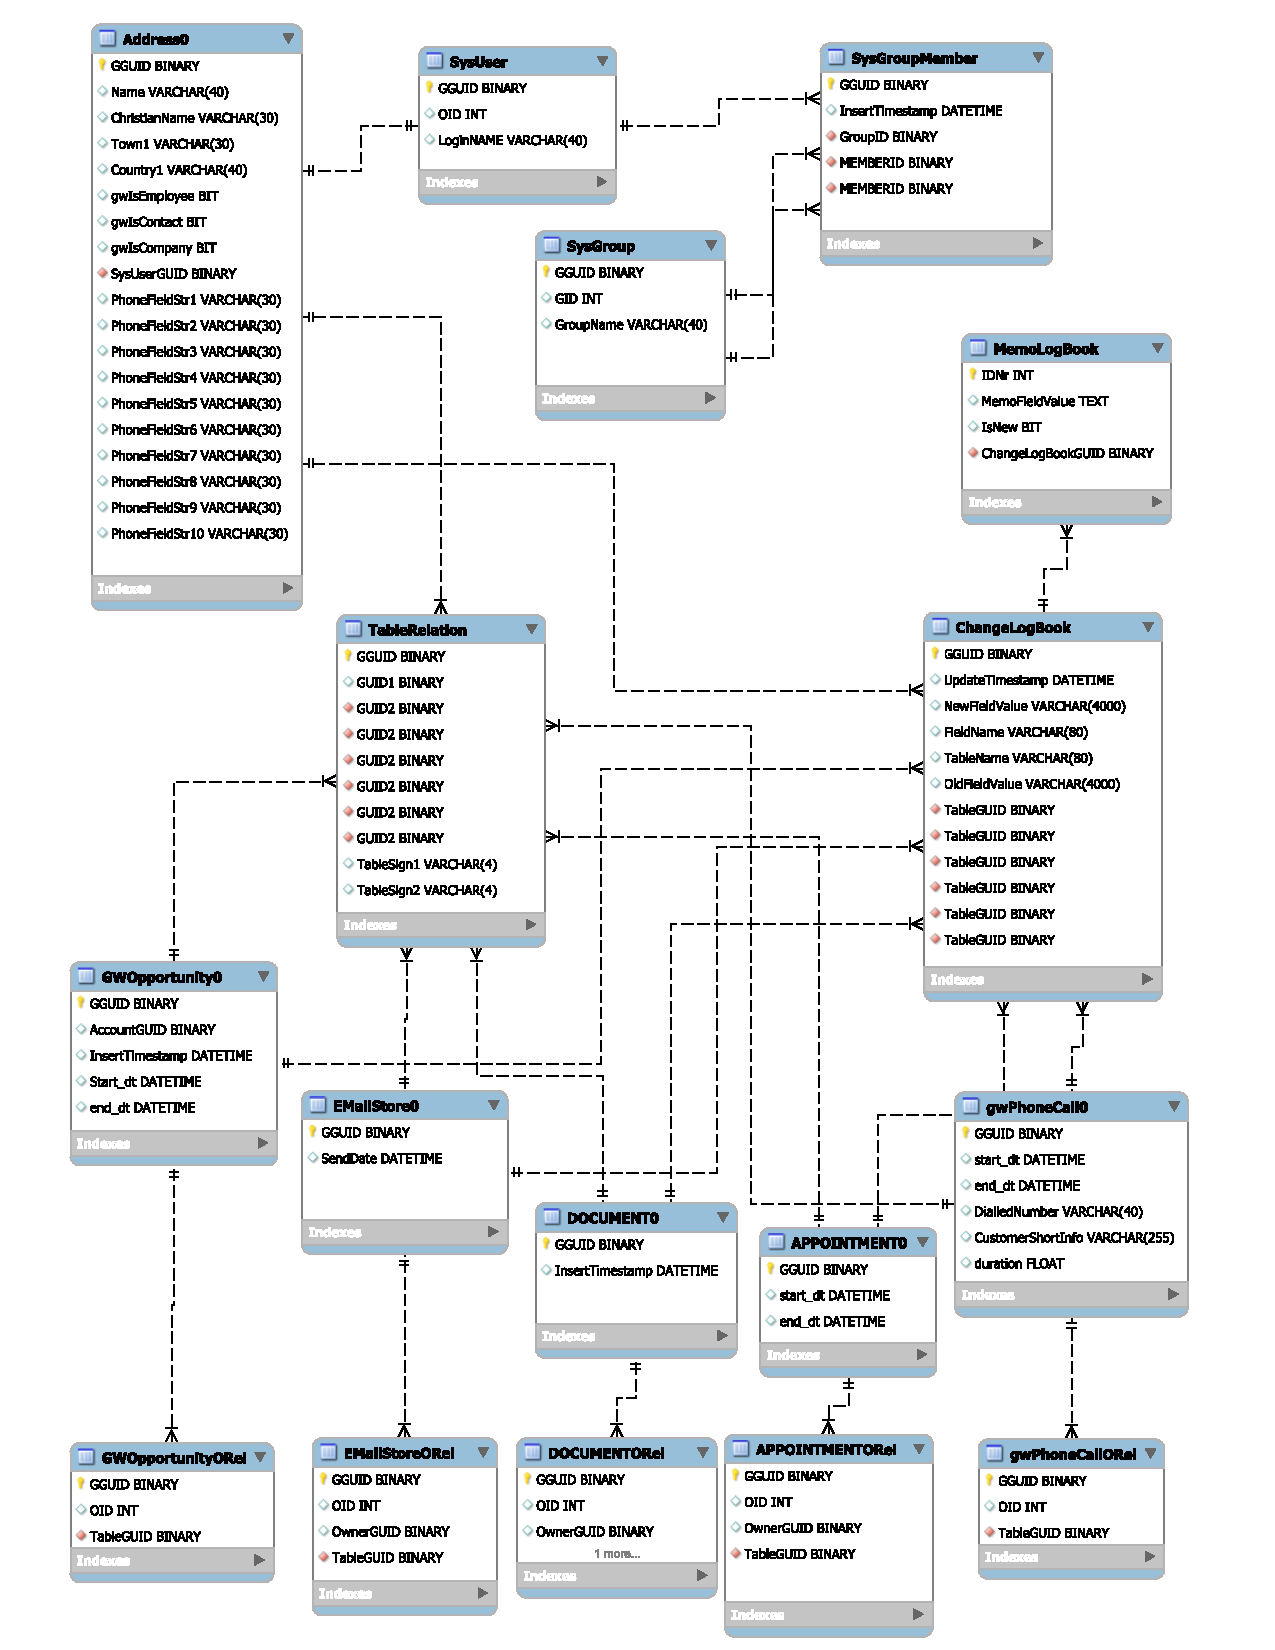
\includegraphics[width=1.0\textwidth]{pics/schema_alt.pdf}
	\caption{Auszug aus dem Schema des MSSQL 2008}
	\label{gw_schema_alt}
\end{figure}

Alle Informationen zu den Verkaufschancen finden sich in der Tabelle \textit{GWOpportunity0}. Die Spalte \textit{InsertTimestamp} wird zum Ermitteln des Erzeugungszeitpunktes benötigt. \textit{start\_dt} und \textit{end\_dt} legen den Zeitraum der Verkaufschance fest. Der Besitzer einer Verkaufschance wird über die Spalte \textit{AccountGUID} bestimmt. Mit den Tabellen \textit{EMailStore0}, \textit{Document0} \textit{Appointment0} und \textit{gwPhoneCall0} verhält es sich wie mit der Tabelle \textit{GWOpportunity0}. Bei der Tabelle\textit{EMailStore0} wird allerdings die Spalte \textit{SendDate} zur zeitlichen Einordnung verwendet. Eine weitere Besonderheit ist in der Spalte \textit{DialledNumber} der Tabelle \textit{gwPhoneCall0} vorhanden. Sie wird zum Vergleich mit der in der Adresse hinterlegten Telefonnummer benötigt. Um festzustellen, ob das Telefonat über einen Tag hinausging wird die Spalte \textit{duration} herangezogen.

Beziehungen lassen sich nicht nur aus der \textit{TableRelation} entnehmen, sondern auch aus den Tabellen die auf \textit{ORel} enden. In ihnen werden  Beziehungen aufbewahrt die durch Teilen von Zugriffsrechten entstanden sind. Jede dieser Tabellen enthält eine \textit{OID} bzw. \textit{GID}, die zur Bestimmung der beteiligten Personen dienen.

Eine Betrachtung basierend auf Zeitspannen impliziert die Veränderung von Zuständen und Konstellationen über die Zeit hinweg. Um diese Änderungen zu erfassen wird die Tabelle \textit{ChangeLogBook} benötigt. Die Spalte \textit{NewFieldValue} enthält die neuen Werte von Tupeln, wohingegen die Spalte \textit{OldFieldValue} den alten Wert besitzt. Die durch die Aktualisierung betroffene Spalte ist in der Spalte \textit{FieldName} hinterlegt. Der Name der betroffenen Tabelle ist der Spalte \textit{TableName} zu entnehmen. Die Referenzierung auf eine Tupel wird in der Spalte \textit{TableGUID} vorgenommen. Aus Gründen des Speicherplatzverbrauchs werden nur varchar Datentypen bei Zeichenfolgen verwendet. Varchar ist allerdings auf 4000 Zeichen limitiert. Falls Zeichenfolgen diese Grenze überschreiten, werden diese in der Tabelle \textit{MemoLogBook} abgelegt. Dort wird der Datentyp Text verwendet, der eine maximale Zeichenfolgenlänge von $2^{31}-1$ (2.147.483.647) erlaubt.
%% ===========================
\chapter{Analyse ausgewählter Datenbanken}
\label{ch:AnalyseDatenbanken}
%% ===========================

Ein Ziel der Bachelor Thesis ist es, hohe Performance in der Beantwortung der Benutzeranfragen zu erreichen. Die maßgebende Komponente ist in diesem Fall die Datenbank. Sie führt die zeitintensiven Ermittlungen, Berechnungen und Filterungen des Gesamtsystems durch. Um Anhaltspunkte für mögliche Kandidaten zu bekommen, sollen im folgenden eine Reihe aus der Literatur bekannte Datenbanken vorgestellt und gegenübergestellt werden. Bei der Zusammenstellung wurde darauf geachtet, dass ein möglichst weites Spektrum unterschiedlicher Datenbanken ausgewählt wurde.

%% ===========================
\section{Datenbanken}
\label{ch:AnalyseDatenbanken}
%% ===========================

Im folgenden werden nun einige aus der Literatur bekannte Datenbanken vorgestellt. Dabei wird insbesondere versucht, einen guten Überblick über die Charakteristika der einzelnen Datenbanken zu geben. Der dahinter stehende Gedanken ist, dass ein späterer Vergleich und Entschluss zur Nutzung besser nachvollziehbar sind. 

%% ===========================
\subsection{CouchDB}
%% ===========================

CouchDB \cite{couch2013} ist eine dokumentenorientierten Datenbank die seit Anfang 2008 unter der  Apache-Lizenz verbreitet wird. In CouchDB werden die Daten in Collections anstatt in Tabellen abgelegt. Collections bestehen aus einer Sammlung von unabhängigen Dokumenten. Jedes Dokument verwaltet seine eigenen Daten in einem freien Schema. 
Ein Dokument hat Feldwerte, die Datentypen (Text, numerisch oder boolean) oder Datenstrukturen (ein Dokument oder Liste) beinhalten. Abfragen werden mit "views" zum Filtern der Dokumente ausgeführt. Indizes sind in CouchDB B-Bäume, so dass die Ergebnisse sortiert und Wertebereich-Anfragen ausgeführt werden können. Abfragen können parallel über mehrere Knoten mit einem MapReduce Mechanismus verteilt werden. CouchDB erreicht Skalierbarkeit durch asynchrone Replikation nicht durch Fragmentierung. Lesezugriffe können auf beliebigen Server stattfinden, wenn Aktualität keine Rolle spielt. Updates hingegen müssen an alle Server weitergegeben werden.
CouchDB unterscheidet sich von anderen Systemen dadurch, dass es Eventual Consistency akzeptiert. Jeder Client erhält eine in sich selbst konsistente Ansicht der Datenbank. CouchDB implementiert Multi-Version Concurrency Control (MVCC) auf einzelne Dokumente mit einer Sequenz-ID die für jede Version eines Dokuments generiert wird. CouchDB benachrichtigt eine Anwendung, wenn jemand anderes das Dokument aktualisiert hat seit dem es zuletzt gefetched wurde. Die Anwendung kann dann versuchen, die Updates zu kombinieren oder das Update zu wiederholen um die Daten zu überschreiben. CouchDB erfüllt damit im lokalen Einsatz die ACID-Eigenschaften. Jede Transaktion ist eine in sich abgeschlossene Operation, die entweder ganz oder gar nicht ausgeführt wird. Es treten keine Seiteneffekte zwischen den Anfragen auf. Außerdem wird die Datenbank immer in einem konsistenten Zustand hinterlassen

%% ===========================
\subsection{MongoDB}
%% ===========================

MongoDB ist ein in C + + geschrieben Open Source Document Store \cite{books/daglib/0025185}. Es hat einige Ähnlichkeiten mit CouchDB. Beide bietet Indizes auf Collections, sie sind lockless, und bieten einen Dokument-Abfragemechanismus. Es gibt jedoch wichtige Unterschiede:

\begin{itemize}

	\item MongoDB unterstützt automatische Fragmentierung die Dokumenten über Server verteilt.
	\item Dynamische Abfragen mit automatischer Verwendung von Indizes werden von MongoDB unterstützt. In CouchDB werden durch das Schreiben von map-reduce views Daten indiziert und gesucht.
	\item CouchDB nutzt MVCC bei Dokumenten, MongoDB hingegen nutzt atomare Operation auf Feldern    

\end{itemize}

MongoDB speichert Daten in einem JSON-ähnlichen binären Format namens BSON. BSON unterstützt boolean, integer, float, Datum, String-und Binär-Typen. Client-Treiber verschlüsseln die lokalen Dokumentendatenstruktur in das BSON Format und senden es an den MongoDB Server. Weiterhin unterstützt MongoDB die GridFS Spezifikation für große binär Dateien wie z.B. Filme oder Bilder. MongoDB unterstützt Master-Slave-Replikation mit automatischem Failover und Recovery. Replikation (und Wiederherstellung) basieren auf dem Prinzip der Fragmentierung. Collections werden über einen benutzerdefinierten Schlüssel automatisch fragmentiert. Die Replikation ist asynchron für höhere Leistung, jedoch können einige Updates bei einem Crash verloren gehen. 

%% ===========================
\subsection{Voldemort}
%% ===========================

Projekt Voldemort \cite{vod2013} ist ein verteilter Key-Value-Store (entwickelt von LinkedIn), der ein hoch skalierbares Speicher-System zur Verfügung stellt. Voldemort repliziert sich durch automatisches partitionieren und anschließendes verteilen der Daten auf multiple Server. Jeder Server stellt einen unabhängigen Knoten im System dar, der für die Verwaltung seiner Daten verantwortlich ist. Dadurch existiert kein Single Point of Failure im Cluster. Ein solches Daten Model erlaubt eine Cluster Expansion ohne eine Neuverteilung der Daten vornehmen zu müssen. In Voldemort können verschiedene Storage Systeme wie BerkeleyDB oder MySQL eingesetzt werden. 

Für die Ablage der Daten werden in Voldemort sogenannte Stores verwendet. Unterstützt werden lediglich Key-Value Ablagen. Jedoch können values komplexere Datenstrukturen wie Maps oder Listen beinhalten. Voldemort stellt 4 verschiedene Operatoren zur Datenmanipulation bereit:

\begin{itemize}

	\item PUT (Key,Value)
	\item GET (Key)
	\item MULTI-GET (Keys)
	\item DELETE (Key, Version) 

\end{itemize}

Eine Möglichkeit für Range Scans ist dabei nicht vorhanden. Der Parameter Version im DELETE-Operator dient der Unterscheidung der Datensätze und ist auf das Verfahren zur Gewährleistung der Konsistenz zurückzuführen. Zur Gewährleistung der eventuellen Konsistenz werden Timestamps und die Vector Clock Technik eingesetzt. Neben der eventuellen Konsistenz bietet Voldemort einen Betrieb mit starker Konsistenz an.       

%% ===========================
\subsection{Redis}
%% ===========================

Redis \cite{red2013} ist ein In-Memory-, Key-Value-Store mit einer Option für Persistenz. Redis Datenmodell unterstützt Strings, Hashes, Listen, Mengen und sortierte Mengen. Obwohl Redis für In-Memory-Daten entworfen wurde, kann je nach Anwendungsfall ein (semi-) persistenter Bestand angelegt werden. Entweder durch Momentaufnahmen der Daten und anschließendes ablegen auf der Festplatte in regelmäßigen Abständen oder durch Aufzeichnen eines Logs mit allen ausgeführten Operationen. Weiterhin kann Redis mit einem Master-Slave-Architektur repliziert werden. Genau wie andere Key-Value-Stores implementiert Redis insert, delete und lookup Operatoren. Weiterhin setzt Redis atomare Updates durch locking um. 

%% ===========================
\subsection{HBase} 
%% ===========================

HBase ist eine verteiltes Open Source Column Store Datenbanksystem welches auf Googles BigTable basiert \cite{Chang:2006:BDS:1267308.1267323}. HBase läuft auf Apache Hadoop und Apache ZooKeeper  \cite{Hunt:2010:ZWC:1855840.1855851} und verwendet das Hadoop Distributed Filesystem (HDFS) \cite{Shvachko:2010:HDF:1913798.1914427}, um Störung-Toleranz und Replikation zu bieten. Zeilen Operationen sind in HBase atomar, mit Sperren auf Zeilenebene und Transaktionen. Partitionierung und Verteilung sind transparent, da es keine Client-Seitiges Hashing oder feste Schlüsselräume wie in einigen NoSQL-Systeme gibt. 
Insbesondere stellt es lineare und modulare Skalierbarkeit sowie streng konsistenten Datenzugriff und automatisches und konfigurierbares Fragmentierung von Daten zu Verfügung. Auf Tabellen können in HBase über eine API zugegriffen werden. Sie können jedoch auch als Ein-und Ausgang Daten für MapReduce-Jobs in Hadoop verwendet werden. Anwendungen speichern in HBase Daten in Tabellen, die aus Zeilen und Spalten Familien bestehen. Spalten Familien beinhalten wiederum Spalten. Darüber hinaus kann jede Zeile einen anderen Satz von Spalten beinhalten. Alle Spalten sind mit einem vom Benutzer bereitgestellten Schlüsselspalte indiziert und in Spalte Familien gruppiert.

%% ===========================
\subsection{Cassandra} 
%% ===========================
Apache Cassandra ist eine verteilte Column Store Datenbank die von Facebook entwickelt wurde \cite{Lakshman:2010:CDS:1773912.1773922}. Sie ist eine Mischung aus Amazon Dynamo und Google BigTable wodurch sie des öfteren als Hybrid zwischen Key-Value-Store und Column Store bezeichnet wird. Cassandra wurde entwickelt um große Daten-Workloads über mehrere Knoten ohne Single Point of Failure zu behandeln. Die Architektur ist von der Annahme geprägt das System-und Hardware-Fehler auftreten können und auch wirklich auftreten. Cassandra behandelt das Problem von Fehlern durch Verwendung eines Peer-to-Peer-System, in dem alle Knoten gleich sind und die Daten von allen Knoten des Clusters verteilt werden. Jeder Knoten tauscht Informationen über das Cluster im Sekunden Takt aus. Ein Commit-Log auf jedem Knoten fängt Schreibaktivität ab um Daten Haltbarkeit zu gewährleisten. Daten werden auch auf eine In-Memory Struktur geschrieben, die memtable. Anschließend in eine Datendatei auf der Festplatte geschrieben genannt SSTable , sobald die Speicherstruktur voll ist. Alle Schreibvorgänge werden automatisch aufgeteilt und in Cluster repliziert. 

Cassandras Datenmodell basiert auf einem partitionierten Row-Store mit variabler Konsistenz. Zeilen werden in Tabellen organisiert, die erste Komponente des Primärschlüssels einer Tabelle ist der Partition Schlüssel. Innerhalb einer Partition werden Zeilen nach den verbliebenen Spalten des Primärschlüssels geclustert. Andere Spalten können getrennt von dem Primärschlüssel indiziert werden. Was Cassandra von HBase unterscheidet sind Spalten, die in einer verschachtelten Weise in Spalte Familien gruppiert werden können. Konsistenz Anforderungen, die zum Zeitpunkt der Abfrage angegeben werden können stellen auch ein Unterscheidungsmerkmal dar. Weiterhin ist Cassandra ein schreiborientiertes System während HBase entwickelt wurde um hohe Leistung für intensive Lese Workloads zu erzielen.

%% ===========================
\subsection{VoltDB} 
%% ===========================

VoltDB \cite{volt2013a} ist ein ACID-konformes relationales In-Memory-Datenbanksystem abgeleitet vom Forschungsprototyp H-Store \cite{kallman08}. Es basiert auf einer Shared-Nothing-Architektur und wurde entwickelt, um auf einem Cluster mit mehreren Knoten zu laufen. Dies wird erreicht indem man die Datenbank in getrennte Partitionen aufteilt bei dem jeder Knoten der Besitzer und Verantwortliche für die jeweiligen Partitionen ist. Durch Verwendung von Stored procedures als Transaktionseinheit, werden Round-Trip-Messages zwischen SQL Anfragen verhindert. Die Anfragen werden seriell in einem einzigen Thread ausgeführt sodass kein locking and latching mehr notwendig ist \cite{volt2013b}. Die Daten werden im Arbeitsspeicher gehalten, was eine Ausführung ohne Netzwerkzugriff und I/O Vorgänge ermöglicht, falls die Daten nur auf einem Knoten liegen.  

%% ===========================
\subsection{H2} 
%% ===========================

H2 ist ein in Java geschriebenes relationales Datenbanksystem, das im Jahre 2004 von Thomas Müller veröffentlicht wurde. Es wird unter der Eclipse Public License verbreitet und ist damit Open Source. H2 bietet neben den festplattenbasierten Tabellen auch eine In-Memory Variante an. Tabellen können dabei dauerhaft oder temporär sein. Weiterhin beherrscht H2 referenzielle Integrität, Transaktionen, Clustering, Datenkompression, Verschlüsselung und SSL. Die Datenbank kann im Embedded- oder Server-Modus betrieben werden.

%% ===========================
\section{Gegenüberstellung} 
\label{ch:AnalyseDatenbanken:sec:Gegenüberstellung}
%% ===========================

Um eine übersichtliche Gegenüberstellung der Datenbanken zu erreichen wurde die Tabelle \ref{tb_charakteristika} angefertigt. Sie enthält vergleichbare Eigenschaften von Datenbanken auf die im folgenden eingegangen wird. 

Die erste Eigenschaft ist das Erscheinungsjahr. Der Grund für die Aufnahme ist das Datenbanken die länger auf dem Markt sind meist eine höhere Reife aufweisen können. Bewährte Datenbanken haben bereits viele Ihrer anfänglichen Probleme behoben was den Umgang mit Ihnen erleichtert. Natürlich sind ältere Systeme nicht frei von Fehlern jedoch existieren für diese viele Workarounds oder andere Lösungsansätze. Cassandra zum Beispiel hat neben zahlreichen Bugfixes über die Jahre CQL als Query Sprache, MapReduce Support, sekundäre Indizies, verbesserte Komprimierung und vieles weiteres erhalten. Es gibt keine feste Regel die besagt wann ein System die Reife für den produktiven Einsatz erreicht hat. Es spielen natürlich auch andere Faktoren bei der Bestimmung der Ausgereiftheit eine Rolle, wie z.B. die Größe des Unternehmens oder Teams das hinter der Datenbank steht. Die Eigenschaft hat weniger den Zweck eines Kriteriums sondern eher eines Indikators. 

Eine wichtige Rolle spielt jedoch die Lizenz unter die Datenbank vertrieben wird. Für Unternehmen ist die Wirtschaftlichkeit eines Systems von großer Bedeutung. Deshalb bieten Open Source Produkte mit ihren geringen Anschaffungskosten trotz des eingeschränkteren Supports einen hohen Anreiz. Neben der Wirtschaftlichkeit sind Möglichkeiten der Manipulation des Source Code ein Pro für Open Source Produkte. 
Kommerzielle Lizenzen bieten hingegen eine höhere Zukunftssicherheit als Open Source Produkte. Sollten die Entwickler der Open Source Produkte keine Lust oder Zeit mehr haben kann die Entwicklung jederzeit eingestellt werden. 

Unterstütze Programmiersprachen und Betriebssysteme sind Eigenschaften bei denen eine Betrachtung des Ist-Zustandes sinnvoll ist. Im Unternehmen sollte optimaler weise schon Erfahrung in Form von Wissen über die verwendeten Technologien vorhanden sein. Externe Mitarbeiter sowie Schulungen sind teuer und müssen bei der Wahl einer für das Unternehmen unbekannte Technologie berücksichtigt werden. 

Die Frage nach ein Schema stellt sich bei einer Betrachtung der Datenstruktur. Wenn sich die Struktur der abzulegenden Daten häufig ändert oder keine einheitliche Struktur unter den Daten zu erkennen ist, sind Schema freie Datenbanken von Vorteil . Durch Schemafreiheit gewinnt man nämlich an Flexibilität. Wohingegen man durch die Nutzung eines Schemas eine bessere Kontrolle der Daten im DBMS besitzt.  


\begin{table}[H]
\tiny
\caption{Gegenüberstellung von den Charakteristika der Datenbanken}
\label{tb_charakteristika}
\setlength{\tabcolsep}{1mm}
\begin{tabulary} {\linewidth} {C | C | C | C | C | C | C | C | C}
\toprule
Eigenschaft & HBase & Cassandra & CouchDB & MongoDB & Redis & Voldemort & VoltDB & H2 \\  
\midrule
Release Datum & 2008 & 2008 & 2005 & 2009 & 2009 & 2009 & 2010 & 2004 \\
\midrule
Datenbankmodell & Wide Column & Wide Column & Document & Document & Key-Value & Key-Value& Relational DBMS & Relational DBMS \\
\midrule
Lizenz & Open Source & Open Source & Open Source & Open Source & Open Source & Open Source & Kommerziell & Open Source \\
\midrule
Server Betriebssysteme & Linux, Unix, Windows & BSD, Linux, OS X, Windows & Android, BSD, Linux, OS X, Solaris, Windows & Linux, OS X, Solaris, Windows & BSD, Linux, OS X, Windows & Linux, Unix, Windows & Linux, OS X & plattformunabhängig \\
\midrule
Daten-schema & schemafrei & schemafrei & schemafrei & schemafrei & schemafrei & schemafrei & ja & ja \\
\midrule
Typisierung & nein & ja & nein & ja & nein & nein & ja & ja \\
\midrule
Sekundärindizes & nein & eingeschränkt & ja (über Views) & ja & nein & nein & ja & ja \\
\midrule
SQL & nein & nein & nein & nein & nein & nein & ja & ja \\
\midrule
APIs und andere Zugriffskonzepte & Java API, RESTful HTTP API, Thrift & Proprietäres Protokoll (CQL) & RESTful HTTP/JSON API & Proprietäres Protokoll basierend auf JSON & Proprietäres Protokoll & Proprietäres Protokoll & Java API, RESTful HTTP/JSON API, JDBC & Java API, ODBC, JDBC \\
\midrule
Unterstützte Programmiersprachen & C, C\#, C++, Groovy, Java, PHP, Python, Scala & C\#, C++, Java, Perl, PHP, Python, Ruby, +5 & C, C\#, Java, JavaScript, Perl, PHP, PL/SQL, Python, Ruby, +9 & C\#, C++, Java, JavaScript, Perl, PHP, Python, Ruby, +4 & C\#, C++, Java, JavaScript, Perl, PHP, Python, Ruby, +12 & C\#, C++, Java, Perl, PHP, Python, Ruby, +8 & C\#, C++, Java, PHP, Python & C\#, C++, Java, PHP, Phyton \\
\midrule
MapReduce & ja & ja & ja & ja & nein & nein & nein & nein \\
\midrule
Konsistenzkonzept & Immediate Consistency & Eventual Consistency, Immediate Consistency & Eventual
Consistency & Eventual Consistency, Immediate Consistency & Eventual Consistency & Strict Consitency, Eventual Consistency &  Integritätsbedingungen & Integritätsbedingungen \\
\midrule
Transaktionskonzept & nein & nein & nein & nein & optimistisches Locking & nein & ACID & ACID \\
\midrule
Nebenläufigkeit & ja & ja & ja & ja & ja & ja & ja & ja \\
\midrule
Embeddable & nein & ja & ja & nein & nein & ja & ja & ja \\
\midrule
In Memory fähig & nein & nein & nein & nein & ja & hybrid & ja & ja \\
\bottomrule
\end{tabulary}
\end{table}

Sekundärindizes sind gerade in Anbetracht der Forderung nach Performance eine interessante Fähigkeit von Datenbanken. Sie erlauben Indizes auf einem oder mehreren Schlüsseln oder Nicht-Schlüsselattributen, was die Effizienz einer Suche steigern kann. Einige NoSQL Datenbank unterstützen solche Indizes wohingegen relationale Datenbanksysteme in der Regel die Definition beliebiger Sekundärindizes erlauben. 

Typisierungen soll zum Ausdruck bringen ob vordefinierte Datentypen wie Float oder Date in der Datenbank vorhanden sind. Ein Vorteil in der Verwendung von Datentypen ist eine Vorabkontrolle der Daten sodass nur Daten mit den entsprechenden Eigenschaften verwendet werden. Zum Nachteil kann die mangelnde Flexibilität ausgelegt werden. Der Nutzer muss wie beim Schema zwischen Flexibilität und Kontrolle entscheiden. 

Die in der Datenbank verwendet Schnittstelle zur Client-Server Kommunikation spielt bei der Architektur des gesamt Systems eine Rolle. Wird der Applikationsserver z.B. auf dem gleichen Server betrieben wie die Datenbank, ist eine Schnittstelle die nur über das Netzwerk angesprochen werden kann nicht sehr sinnvoll. Wird die Datenbank hingegen über das Netzwerk von eventuell mehreren Servern angesprochen, so eignet sich der Einsatz von REST-Protokollen. 

Die Entscheidung ob eine gewisse Stärke der Konsistenz ausreichend ist wird durch den Anwendungsfall bestimmt. In manchen Anwendungen ist es schlichtweg egal ob Daten redundant sind oder nicht. Die darüberliegende Anwendungsschicht muss bei Inkonsistenz damit rechnen sonst kann es zu schwerwiegenden Fehlern kommen. Beim Transaktionskonzept verhält es sich wie bei der Konsistenz, es hängt vom Anwendungsfall ab. Nebenläufigkeit gibt lediglich an ob gleichzeitig ausgeführte Datenmanipulation durch die Datenbank unterstützt wird.   

Ob eine Datenbank im Embedded Modus betrieben werden kann ist von Bedeutung wenn eine Integration in die Anwendung gewünscht ist. Dadurch können z.B. Verzögerungen durch Netzwerkzugriffe bei der Datenabfrage vermieden werden. 

Die Eigenschaft In Memory spiegelt den Wunsch der CAS Software AG wieder. Sie stellt somit einen der wichtigsten Kriterien für die Auswahl der Datenbank dar.

%% ===========================
\section{Ergebnisfindung}
\label{ch:AnalyseDatenbanken:sec:Ergebniss}
%% ===========================

Jede Datenbank hat seine eigenen Stärken und Schwächen. Bei der Wahl der passenden Datenbank ist nicht entscheiden welche Datenbank im Vergleich zur anderen die Beste ist. Vielmehr ist von entscheidender Bedeutung ob die entsprechende Datenbank den Anforderungen an das Gesamt System gerecht werden kann. 

Dementsprechend ist in diesem Anwendungsfall die Performance einer Datenbank am bedeutsamsten. Die Verwendung des Hauptspeichers als Primärspeicher bedeutet einen theoretischen Geschwindigkeitsvorteil um den Faktor 100.000. In der Realität ist dieser Faktor meist zwar nicht zu erreichen jedoch ergibt sich für Datenbanken die dies ausnützen können ein Vorteil gegenüber anderen. Fünf der Neun Datenbanken bieten diese Möglichkeit nicht. Deswegen ist zu klären ob diese Datenbanken andere Charakteristiken aufweisen können um diesen Nachteil auszugleichen.

Cassandra und HBase ermöglichen hohe Performance durch horizontale Skalierung. Sie erlauben es durch hinzunahmen von Servern zusätzliche Leistung zu erzielen. Die Kunden der CAS Software AG sind alles mittelständische Unternehmen, welche nicht an die Nutzerzahlen von Facebook und Google herankommen. Daher sind wenige Zugriffe zu erwarten. Vorteile durch mögliche horizontale Skalierung fallen somit weg. Es ist zu erwarten das Cassandra und HBase auf einzelnen Servern nicht an die Performance von In Memory fähigen Datenbanken herankommen. Dies führte zu einer Entscheidung gegen die beiden Vertreter der Wide Column Stores.

Die Document Datenbanken sind zwar auch horizontal Skalierbar kommen jedoch nicht an die Performance von beiden zuvor genannten Datenbanken heran. Ihre Stärke liegt in Ihrer Schema freien Datenhaltung die an dieser Stelle von geringem Wert ist da die Daten eine feste Struktur haben. Außerdem sind Funktion wie SUM werden nicht in der eigenen API mitgeliefert was sie für analytische aufgaben bedingt brauchbar macht. Letztendlich können die CouchDB und MongoDB nicht überzeugen weshalb sind ebenfalls nicht verwendet wurden.

Die Key-Value-Stores ermöglichen mit Ihrer Form der Datenhaltung und der In Memory Fähigkeit hohe Zugriffsgeschwindigkeiten. Was Ihnen jedoch zum Nachteil ausgelegt werden muss ist Ihre mangelnde Komplexität. Sie sind besonders für Punkt Abfragen geeignet. Komplexe Anfragen sind nur durch deren Realisierung in der Logikschicht möglich. Was einen enormen Aufwand mit sich bringen würde. Daher entschied man sich auch gegen die Key-Value-Stores. 

VoltDB ist von den Eigenschaften her ein optimaler Kandidat allerdings nicht Open Source. Die Datenbank konnte dadurch nicht verwendet werden. H2 hingegen ist Open Source und bietet Optionen zum Vorhalten der Tabellen im Hauptspeicher. Davon erhofft man sich hohe Geschwindigkeitsvorteile gegenüber herkömmlichen relationalen Systemen. Durch den Ansatz der relationalen Algebra ist das Arbeiten mit SQL möglich. Das birgt Vorteile da auf bereits bekanntem Wissen aufgebaut werden kann.
%% content.tex
%%

%% ===========================         
\chapter{Konzeption}
\label{ch:Konzeption}
%% ===========================

Ein Konzept dient in der Softwarearchitektur der Konstruktion eines abstrakten Systemmodells. Zur Gestaltung werden technische Details weggelassen und stattdessen allgemeingültige Begriffe und ihre Zusammenhänge festgelegt. Weiterhin wird ein Grundverständnis durch Definieren von Strukturen und Konzepten gebildet. Darüber hinaus werden Schnittstellen definiert, die Wechselwirkungen zwischen den Komponenten beschreiben. Weiterhin werden im Zuge der Überlegungen Technologien ausgewählt, die zur Umsetzung der verschiedenen Komponenten verwendet werden. Abschließend wird auf die Entwürfe der einzelnen Komponenten näher eingegangen.  

%% ===========================
\section{Architektur}
%% ===========================

Zuerst wird ein erster Überblick über den geplanten Aufbau des Systems gegeben. Abbildung \ref{konzept_architektur} zeigt die Komponenten des Systems und der Umwelt. Der Tomcat mit seinen Webcontainern bildet die Basis des Systems. Wie auf der Abbildung zu sehen sind zwei verschiedene Projekte vorgesehen. Zum einen ein Client-Webprojekt und zum anderen ein Server-Webprojekt. Das Client-Webprojekt soll die Klassen und Methoden zur Umsetzung der Darstellung beinhalten. Die Anwendungslogik sowie die Datenbank sind im Server-Webprojekt vorgesehen. Der Grund für die Aufteilung in zwei verschiedene Webprojekte ist die Anforderung einer losen Kopplung zwischen Client und Server. Beide Webprojekt werden in Form von Web-Archive-Dateien in einem Apache-Tomcat-Webserver deployed und können über die entsprechende URL angesprochen werden. Weiterhin soll ein selbstgeschriebenes Plugin für den CAS genesisWorld Anwendungsserver die Aktualität des Systems garantieren. Der Browser, CAS genesisWorld und der MSSQL-Server stellen die Umwelt des Systems dar. Im Folgenden wird auf jede Komponente der Architektur eingegangen und ihre Rolle im Gebilde erläutert.

\begin{figure}[htbp]
\centering
  \includegraphics[width=0.8\textwidth, width=0.8\textwidth]{pics/Konzept_architektur.pdf}
\caption{Komponenten des Systems und der Umwelt}
\label{konzept_architektur}
\end{figure} 

\paragraph{Vaadin Client-Side-Engine}

Die Vaadin Client-Side-Engine verwaltet das Rendering der Oberfläche im Web-Browser.  Dies geschieht durch den Einsatz verschiedener clientseitiger Widgets, die das Gegenstück zu den serverseitigen Vaadin-Komponenten bilden. Es leitet Benutzerinteraktionen an die Serverseite weiter und rendert anschließend die Änderungen für die Benutzeroberfläche. Die Kommunikation findet über asynchrone HTTP-oder HTTPS-Anfragen statt. Weiterhin wird die Komponente durch Vaadin automatisch erzeugt und wird daher als gegeben betrachtet.

\paragraph{Client-Webprojekt}

Die Oberfläche des Systems wird durch ein Vaadin-Projekt realisiert. Mit dessen Hilfe werden die Bedien- und Darstellungselemente der Anwendung definiert. Sie ist außerdem für die Interaktion mit dem Benutzer zuständig. Die Delegation von verschiedenen Clients beispielsweise wird von einem Vaadin-Servlet erledigt. Dazu zählt das Empfangen von Anfragen und deren Zuordnung zu einer Sitzung des jeweiligen Benutzers. Die Elemente der Oberfläche selbst werden in Java geschrieben. Mithilfe der Java-Klasssen wird zur Laufzeit eine Javascript basierte Homepage erzeugt. Den Übergang von Java auf Javascript übernimmt Vaadin.

Das Server-Webprojekt ist eine weitere Komponente mit der interagiert werden soll. Die Kommunikation zwischen den beiden Komponenten soll über das REST-Protokoll stattfinden. Dazu implementiert das Client-Webprojekt einen REST-Client. Die Verwendung des REST-Protokolls zwischen dem Client-Webprojekt und Server-Webprojekt stellt überdies einen weiteres Element der losen Kopplung dar.

Ein Prozess in dem die einzelnen Bestandteile Verwendung finden, könnte wie folgt aussehen: Die Interaktionen der Benutzer mit der Oberfläche würden Events erzeugen, die zunächst auf der Clientseite durch Widgets verarbeitet werden. Nachfolgend würden die Events durch den HTTP-Server an das Vaadin-Servlet übergeben werden. Dieser leitet die Events an die entsprechenden Vaadin-Objekte weiter, bis sie zu den in der Anwendung definierten Event-Listenern gelangen. In den Listenern werden anschließend die REST-Clients aufgerufen. Mit Hilfe der REST-Clients werden die Eingaben der Nutzer an das Server-Webprojekt übermittelt. 

\paragraph{Server-Webprojekt}

Die eigentliche Lösung der Problemstellung soll im Server-Webprojekt des Softwaresystems implementiert werden. Es soll vollständig auf Java basieren. In ihr werden sich Klassen und Methoden befinden die eine Ermittlung der Informationen aus der H2-Datenbank ermöglichen. Zur Bestimmung der SQL-Parameter soll ein REST-Server implementiert werden, der die Beinutzeingaben entgegennimmt. Der REST-Server ist außerdem für die Kommunikation mit dem Plugin zuständig.

Weiterhin soll das Projekt sämtliche ETL-Prozessschritte implementieren. Die genaue Vorgehensweise des Prozesses wird in Abschnitt \ref{ch:konzeption:etl} behandelt. 

%Die Logikkomponente in der Architektur stellt eine Zusammenfassung aller Funktionen des Anwendungskerns dar. Sie kümmert sich um die Generierung der Abfragen, welche an die Datenbank gestellt werden. Dabei erfolgt eine dynamische Generierung der Abfragen, um nicht durch unnötige Bedingungen die Verarbeitungsgeschwindigkeit zu verringern. Abfragen werden mithilfe der Java Database Connectivity (JDBC) an die Datenbank gestellt. Neben den Funktionen zur Abfragegenerierung enthält die Logikkomponente Prozesse zum Extrahieren und Transformieren von Daten aus der MSSQL-Datenbank. Der ETL-Prozess wird nur einmalig ausgeführt, allerdings stellt er einen wichtigen  Schritt für die Umsetzung dar. 


%In der Server.war werden REST-Requests entgegen genommen. Anhand der mitübertragenen Filteroptionen werden die Bedingungen für die Datenbankabfrage zusammengestellt. Anschließend wird eine Verbindung zur H2-Datenbank aufgebaut. Das Ergebnis der Abfrage wird in das JSON-Format überführt und zurück an die Client.war geschickt. Dort angekommen werden die Daten an die Vaadin-Komponenten übergeben, was einen Neuaufbau der entsprechenden Seitenbereiche bewirkt.      

\paragraph{H2-Datenbank}

Die H2-Datenbank ist als Teil des Server-Webprojektes geplant. Dies wird durch den Betrieb im Embbeded-Modus ermöglicht. Dadurch kann direkt aus dem Java-Code heraus mit der Datenbank gearbeitet werden. Um möglichst kurze Antwortzeiten zu Erreichen soll die In-Memory-Variante der Tabellen verwendet werden.

\paragraph{CAS genesisWorld Plugin} Systeme die auf dem Datenbestand anderer Systeme aufbauen können zwei verschiedene  Ansätze zur Sicherstellung ihrer Aktualität verfolgen. Unser nebenläufiges System bezeichnen wir als A und den CAS genesisWorld Anwendungsserver als B. Einer der Ansätze ist die Intervall basierte Nachfrage über Veränderungen von A. Hierbei fragt A bei B zu festgelegten Zeitpunkten nach, ob Daten verändert wurden. Die Definition eines optimalen Intervalls stellt eine der größten Schwierigkeiten dar. Ist der Intervall zu groß, sinkt die Aktualität des Datenbestandes. Ist er zu klein, entsteht eine starke Belastung für B. Der andere Ansatz ist A über Veränderungen an den Datensätzen von B zu informieren. Dadurch werden keine unnötigen Abläufe angestoßen, da nur im Falle einer Manipulation eines Datensatzes Prozesse in Bewegung gesetzt werden. Zwar wird die Aktualität der Daten gewährleistet, jedoch büßt A an Entscheidungsfreiheit ein. A kann nicht mehr selbst entscheiden wann aktualisiert wird. Der zweite Ansatz ist zwar effizienter, allerdings nicht immer umsetzbar. Das kann technische oder unternehmenspolitische Gründe haben, die notwendige Veränderung am Legacy-Systems ausschließen.  

In CAS genesisWorld gibt es die Möglichkeit den zweiten Ansatz umzusetzen. Die Idee dabei ist den CAS genesisWorld Anwendungsserver um ein Plugin zu erweitern, welches über Veränderungen in den Datensätzen benachrichtigt wird. Das Plugin soll über einen REST-Client die \textit{GGUID} des betroffenen Datensatzes an den Server-Webprojekt senden. Dort soll eine Kontrolle stattfinden, die den Datensatz auf Relevanz überprüft. Wird eine Relevanz festgestellt besorgt sich das Server-Webprojekt, anhand der zuvor übermittelten GGUID, alle benötigten Daten.

%% ===========================
\section{Datenbankdesign}
%% ===========================

Das Datenbankdesign stellt einen wichtigen Abschnitt der Konzeption dar. An dieser Stelle werden Festlegungen im Bereich des Datenmodells getroffen. Sie entscheiden, ob Anforderungen und Erwartungen erfüllt werden können. Weiterhin werden die Charakteristika der Daten untersucht und das Datenmodell entsprechend nach ihnen ausgelegt.

%% ===========================
\subsection{Konzeptionelles Design}
%% ===========================

Zunächst wird auf das geplante Schema der H2-Datenbank eingegangen. Indessen werden die Überlegungen und Gründe die zur Entstehung des Schemas geführt haben erläutert. 

Die Normalisierung dient der Organisation von Feldern und Tabellen einer relationalen Datenbank, um Redundanz und Abhängigkeit zu minimieren. Die Kehrseite hingegen, ist eine Steigerung des Aufwands, um die benötigten Daten wiederzugewinnen. Normalisierung bietet dem Designer die Möglichkeit einen Austausch zwischen Performance und Stabilität des Datenbankmodells vorzunehmen. 
In diesem Fall stellt ersteres absolute Priorität dar. Daher soll die Normalisierung so gering wie möglich gehalten werden. 

Die erste Überlegung hinsichtlich des Schemas führt zu der Frage, welche Daten zur Umsetzung des Systems benötigt werden. Der Datenbankdesigner steht bei analytischen System immer wieder vor der Entscheidung, wie viele Informationen aus dem alten System in das neue System übernommen werden sollten. Um höchstmögliche Verarbeitungsgeschwindigkeiten zu erreichen, werden lediglich die für das Szenario benötigten Daten extrahiert. Abbildung \ref{konzept_SchemaNeu} zeigt das für die Datenbank neu entworfene Schema. 

\begin{figure}[htbp]
\centering
  \includegraphics[width=0.8\textwidth, width=0.8\textwidth]{pics/NewSchema.pdf}
\caption{Neues Datenbankschema}
\label{konzept_SchemaNeu}
\end{figure} 

Die Idee hinter dem Schema ist die Verwendung einer einzelnen Tabelle zur Aufbewahrung der Informationen über die Verbindungen zwischen den Beziehungen. Diese Tabelle ermöglicht es ausgehend von einer Person alle Verbindungen die zu anderen Personen führen herauszufinden. Im Grunde genommen sind vier Spalten dafür ausreichend. Die erste Spalte \textit{startID} beinhaltet die Person von der die Suche ausgeht. Eine Zuordnung der Tupel zu einem Datum erfolgt über die Spalte \textit{Date}. Um Verbindungsmerkmale zu unterscheiden, werden Zahlen von eins bis fünf für die jeweiligen Verbindungsmerkmale in der Spalte \textit{DataTyp} verwendet. Die letzte Spalte \textit{endID} beinhaltet die ID von Personen, zu denen die Verbindungen letztendlich führen. Alle anderen Spalten wie z.B. \textit{Town} oder \textit{Country} dienen der Filterung von Abfragen.

Um mit den geringeren Speicherkapazitäten des Hauptspeichers zurechtzukommen, wird auf das Problem der Datenredundanz eingegangen. Durch Normalisierung lässt sich Datenredundanz zwar nicht verringern, allerdings kann man sie in kontrollierbare Bahnen lenken. Im neuen Schema werden solche Maßnahmen auf die Spalte \textit{Town} und \textit{Country} angewendet. 

Die Spalte \textit{Country} beispielsweise wird voraussichtlich Millionen von Werten beinhalten, jedoch gibt es nur eine Hand voll Länder auf der Welt. Die Ländernamen werden sich daher sehr oft wiederholen. Der Datentyp Varchar benötigt pro Zeichen 2 Byte an Speicherplatz. Aufgrund der stetigen Wiederholung von gleichen Wörtern ist die Verwendung von Varchar an dieser Stelle ungeeignet. Angesichts dessen werden die Ländernamen in einer eigenen Tabelle aufbewahrt. In dieser wird jedes Land nur einmal vermerkt und bekommt einen Primärschlüssel in Form einer Zahl. In der Tabelle \textit{Data} wird dann nur noch der jeweilige Fremdschlüssel verwendet. Das würde zum Beispiel bei dem Wort "Deutschland" eine Reduktion von 22 Byte auf 1 Byte bewirken. Die Reduzierung auf 1 Byte entsteht durch die Verwendung des Datentyps tinyint. Das alles gilt ebenfalls für die Spalte \textit{Town}. Bei ihr wird allerdings der Datentyp smallint verwendet, da dessen Zahlenbereich von -32768 bis 32767 reicht. Damit lassen sich alle Städte aus dem MSSQL-Server abdecken. 

Die Spalten \textit{isEmployee}, \textit{isContact} und \textit{isFirm} können nur zwei verschiedene Zustände darstellen. Trifft zu oder trifft nicht zu. Der Datentyp \texttt{bool} reicht daher zur Abbildung der zweiwertigen Zustände aus. Ein Feld vom Datentyp datetime benötigt 8 byte an Speicher. Um hier ebenfalls Einsparungen vorzunehmen, wurde beschlossen das Datum als smallint zu deklarieren. Dies ist möglich, weil nur der Tag innerhalb des Datums von Interesse ist. Dazu wird ein frei gewählter Nullpunkt festgelegt. In unserem Fall wurde der 01.01.1990 als Nullpunkt gewählt, da keine älteren Daten existieren, die Relevanz besitzen. Der Wert eines Datum wird durch die Anzahl der Tage seit dem Nullpunkt ermittelt. Dieser Wert wird anschließend in der Spalte \textit{Date} abgelegt. Die Hochrechnung der Tabelle \ref{tb_speicherplatzverbrauch} zeigt, dass durch die Normalisierung der Speicherplatzverbrauch um bis zu $ \frac{1}{6} $ gesenkt werden kann.

\begin{table}[htbp]
\centering
\begin{tabulary} {\linewidth} {l  r  C  l  C  r}
& & & & & \\
\multicolumn{6}{l}{Speicherplatzverbrauch ohne Normalisierung}\\
& & & & & \\
Zeitpunkt(timestamp) & 8 byte & x & 18.000.000 & = & \textasciitilde 137 MB \\  
Stadt(varchar) & 16 byte & x & 18.000.000 & = & \textasciitilde 343 MB \\  
Land(varchar) & 20 byte & x & 18.000.000 & = & \textasciitilde 274 MB \\  
\midrule
& & & & Summe & \textasciitilde 754 MB\\
& & & & & \\
\multicolumn{6}{l}{Speicherplatzverbrauch mit Normalisierung}\\
& & & & & \\
Zeitpunkt(smallint) & 2 byte & x & 18.000.000 & = & \textasciitilde 34 MB \\  
Stadt(integer) & 4 byte & x & 18.000.000 & = & \textasciitilde 72 MB \\  
Stadt(varchar) & 16 byte & x & 21.000 & = & \textasciitilde 0,32 MB \\  
Land(tinyint) & 1 byte & x & 18.000.000 & = & \textasciitilde 17 MB \\  
Land(varchar) & 20 byte & x & 218 & = & \textasciitilde 0,004 MB \\
\midrule  
& & & & Summe & \textasciitilde 123 MB\\
& & & & & \\
\end{tabulary}
\caption{Vergleich des Speicherplatzverbrauchs}
\label{tb_speicherplatzverbrauch}
\end{table}

Wird eine Benutzerabfrage gestellt die eine Filterung anhand einer Stadt voraussieht, wird zuerst die \textit{ID} der Stadt benötigt. Dabei können zwei verschiedene Ansätze verfolgt werden. Der erste Ansatz wäre ein Verbund zwischen \textit{Town} und \textit{Data}, um direkt mit dem Namen der Stadt zu arbeiten. Diese Variante dürfte aufgrund des Kreuzproduktes von Millionen von Zeilen nicht sehr performant sein. Eine andere Möglichkeit wäre eine separate Abfrage an die Datenbank zu stellen, in der die \textit{ID} zum Namen ermittelt wird. Mithilfe der \textit{ID} kann dann ohne einen Verbund die Ergebnismenge ermittelt werden. Dieser Ansatz dürfte vor allem durch die Abwesenheit von Netzwerkzugriffen zu geringeren Antwortzeiten führen. Dieses Vorgehen kann für die Stadt, das Land und die Gruppenzugehörigkeit angewendet werden.


Die Tabelle \textit{GroupDate} unterscheidet sich von den anderen Tabellen wie \textit{Town} oder \textit{Country}, da in dieser noch weitere Details vermerkt sind. Diese ermöglichen es die Zusammenstellung von Gruppen über die Zeit nachzuvollziehen. In der Spalte \textit{Action} wird festgelegt, ob die Tupel einen Eintritt oder einen Austritt einer Person darstellt. Die Spalte \textit{Date} beinhaltet das Datum des Ereignisses. Mithilfe beider Attribute lassen sich Gruppenzusammensetzung auf bestimmte Zeitpunkte bezogen rekonstruieren.

%% ===========================
\subsection{Zugriffsstrukturen}
%% ===========================

Zum Beschleunigen der Zugriffe auf die Datensätze der H2-Datenbank wird auf die beabsichtigten Zugriffsverfahren eingegangen. 

Indizes werden zur Beschleunigung von Suchen nach bestimmten Spaltenwerten eingesetzt. Ohne Indizes müsste die H2-Datenbank beim ersten Datensatz beginnen und dann die gesamte Tabelle durchgehen, um eine Abfrage zu beantworten. Je größer die Tabelle ist, desto höher sind die Kosten dafür. Der Einsatz von Indizes ist in Anbetracht der Zielsetzung von niedrigen Antwortzeiten ein interessantes Hilfsmittel. Jeder Index bedeutet allerdings einen Zuwachs im Speicherplatzverbrauch. Zur Indexierung der Tabellen \textit{Town}, \textit{Country}, \textit{User} und \textit{Group} eignen sich Hash-Indizes. Sie bieten einen extrem schnellen Zugriff auf die Daten. Diese Schnelligkeit ergibt sich aus der Verwendung von Berechnungsvorschriften, zur Ermittlung der Position des gesuchten Wertes. Indizierungen sollen im vorliegenden Schema über die Spalten mit der Bezeichnung \textit{Name} vorgenommen werden, da der Client mit dem Namen anstatt mit der ID arbeitet. Mithilfe des Namens wird deshalb die zugehörige ID ermittelt. Die Nutzung von Hash-Indizes bringt allerdings Limitierungen mit sich. Eine der wichtigsten ist, dass sie nur für Vergleiche ("=") verwendbar sind. Somit werden keine Wertebereichabfragen ("<" oder ">") unterstützt. Es gibt allerdings noch andere Nachteile \cite{SWB-352401869}, auf die aber in dieser Arbeit nicht näher eingegangen wird. 

Für die Tabelle \textit{UserGroup} eignet sich der B\textsuperscript{+}-Baum-Index von H2. Dieser kann für die Spalte \textit{userID} verwendet werden, der den ersten Wert einer Suche darstellt. Der B\textsuperscript{+}-Baum-Index eignet sich auch für die Tabelle \textit{Data}. Hier ist außerdem die Verwendung eines Mehr-Attribut-Indexes vorgesehen. Der Vorteil eines Mehr-Attribut-Indexes ist, dass bei einer Punkt-Abfrage über alle Zugriffsattributwerte nur ein Indexzugriff erfolgen muss. Indexiert werden in unserem Fall die Spalte \textit{startID} und \textit{Date}. Beide Spalten sind sortiert und bieten sich somit für die Verwendung eines geclusterten Index an. Geclusterte Indizes sind in der gleichen Form sortiert wie die interne Relation. Ein geclusterter Index unterstützt Bereichsanfragen sehr gut, was bei der Beschränkung auf Zeitspannen von Vorteil sein dürfte.       


%% ===========================
\section{Extract Transform Load Prozess}
\label{ch:konzeption:etl}
%% ===========================

Daten der operativen Systeme unterstützen die wertschöpfenden Geschäftsprozesse innerhalb eines Unternehmens. Sie sind demnach auf die Steuerung und Überwachung des Tagesgeschäftes ausgerichtet und daher transaktionsbezogen. Somit sind die Daten in ihren Begrifflichkeiten häufig nicht vergleichbar und ihrer Bewertung sowie Konsolidierung unterschiedlich. Um die Daten dennoch für analytische Zwecke einzusetzen, ist eine Überführung in eine geeignete Struktur von Vorteil. Eine solche Überführung wird in der Literatur als Extract-Transform-Load (ETL)-Prozess bezeichnet \cite{ElSappagh201191}. 

Abbildung \ref{konzept:etl} zeigt das erarbeitete Konzept zur Umsetzung des ETL-Prozesses. In den nächsten drei Abschnitten wird jeder ETL-Schritt näher erläutert.

\begin{figure}[htbp]
\centering
  \includegraphics[width=1.0\textwidth, width=1.0\textwidth]{pics/ETL.pdf}
\caption{ETL-Prozess}
\label{konzept:etl}
\end{figure} 


%% ===========================
\subsection{Extract}
%% ===========================

Zunächst dient die Extraktion primär der Beschaffung von Daten aus dem MSSQL Server. Überdies können durch den Prozess Daten bereits reduziert,  zusammengeführt und ersetzt werden. Für eine zutreffende Formulierung der Abfragen müssen Besonderheiten in die Ermittlung der Daten beachtet werden. Eine vollständige und korrekte Datenmenge stellt die Grundlage jeder guten Analyse dar.

Die erste Besonderheit stellt die Beachtung des zeitlichen Aspekts in der Extraktion dar. Es gilt dabei die Veränderungen der Daten über die Zeit zu berücksichtigen. Die Tabelle  \textit{Changelogbook} ermöglicht es Änderungen in den Datensätzen nachzuvollziehen. Eine solche Veränderung ist in der Gruppenzusammensetzung zu finden, die sich aufgrund von Abgängen und Zugängen von Personen ändert. Neben den Datensätzen die sich über die Zeit verändern, existieren Datensätze die sich über längere Zeiträume erstrecken. Beispielsweise erstrecken sich Termine wie Tagungen  über mehrere Tage. In der MSSQL-Datenbank werden diese Termine in einer Tupel aufbewahrt. Bei unserer Analyse hingegen stellt jede Tupel eine Verbindung zu einem bestimmten Tag dar. Somit muss ein Datensatz der sich über mehrere Tage erstreckt, in der H2-Datenbank durch mehrere Tupeln repräsentiert werden. Aufgrund dessen wird im Ergebnis der SQL-Abfrage die Anzahl der Tage vermerkt. In späteren Transformationen kann mithilfe dieser Angaben die entsprechende Anzahl an Tupeln erzeugt werden.

Eine weitere Besonderheit ergibt sich durch eine Funktionalität von CAS genesisWorld CAS, welche es ermöglicht Termine zu schieben. Diese Funktion wird von manchen Nutzern missbraucht. Anstatt für einen ähnlichen Termin einen neuen Eintrag anzulegen, wird ein alter Termin aus Bequemlichkeit geschoben. Das hat zur Folge, dass Termine die tatsächlich stattgefunden haben, in der Datenbank nicht mehr existieren. Um trotzdem diese Termine zu berücksichtigen wurde folgendes Konzept erarbeitet. Dem \textit{Changelogbook} lassen sich Veränderungen von Feldern entnehmen. Um Schiebungen zu erkennen werden die Änderungen in den Spalten \textit{start\_dt} und \textit{end\_dt} benötigt. 

Zur Feststellung ob ein Termin stattgefunden hat und anschließend geschoben wurde, müssen drei Bedienungen erfüllt sein. Die erste ist der Zeitpunkt der Schiebung, der nach dem Termin liegen muss. Wird ein Termin aus anderen Gründen geschoben findet dies in der Regel vor dem Start des Termines statt, damit die Personen nicht unnötig zum Termin erscheinen. Die zweite Bedingung ist, dass der neue Termin in der Zukunft liegen muss. Neben den beiden zuvor genannten Bedingungen muss die Operation auf den Datensätzen ein Update gewesen sein. Nur dann ist der Datensatz von Relevanz für die Abfrage. 

Die Ergebnisse sämtlicher Extraktionen werden in CSV-Dateien abgespeichert. Damit werden unteranderem eventuelle Fehlersuchen vereinfacht. Weiterhin wird die Belastung des Hauptspeichers verringert, da nicht alle Ergebnisse bis zum Ende der Extraktion in der Java-Laufzeitumgebung aufbewahrt werden müssen.

%% ===========================
\subsection{Transform}
%% ===========================

Zu Beginn der Transformation werden Filterungen durchgeführt. Unter der Filterung von operativen Daten versteht man eine Bereinigung syntaktischer oder inhaltlicher Defekte, der zu übernehmenden Daten. Die MSSQL-Datenbank besteht zu 37\% aus Nullwerten und zu 4\% aus leeren Feldern. Daten die beispielsweise Nullwerte enthalten und für die Ermittlung des Datums benötigt werden, sind für die Analyse nicht zu gebrauchen. Sie können daher im Laufe des Prozesses aus den Daten entfernt werden. Bei den anderen Filteroperationen können Nullwerte vernachlässigt werden, da sie zweckmäßig abdingbar sind.

Der nächste Schritt ist die Harmonisierung der Daten. Unter anderem besitzen die Telefonnummern kein einheitliches Format. Sie wurde manuell von Sachbearbeitern eingetragen. Zur Lösung des Problems werden aller Nummern in ein einheitliches Format gebracht, welches einen automatischen Vergleich ermöglicht. Die Verbindungsmerkmale müssen ebenfalls in eine einheitliche Form gebracht werden. Spalten die gleiche Inhalte besitzen, aber unterschiedlich bezeichnet sind, müssen unter einer Bezeichnung zusammengeführt werden. 

Die in der Extraktion genannten Besonderheiten werden durch unterschiedliche Datenbankabfragen ermittelt. Dies führt zu vielen separaten Dateien. Zur Nutzung der Daten sind diese zum Abschluss der Transformation zusammenzuführen. Das Ergebnis wird anschließend in einer CSV-Datei gespeichert, welche die Basis zum Einspielen der Daten in die H2-Datenbank bildet. 

%% ===========================
\subsection{Load}
%% ===========================

Beim Laden der Datensätze in die H2-Datenbank kommt ein sogenannter "bulk load" zum Einsatz. Dieser wird häufig zum Laden von großen Datenmengen aus einer Datei in eine Datenbank eingesetzt. Er ermöglicht ein wesentlich schnelleres einspielen von großen Datenmengen in die Datenbank, gegenüber der Verwendung von INSERT-Operatoren.

%% ===========================
\section{Darstellungskonzepte}
\label{ch:Konzeption:sec:Darstellungskonzepte}
%% ===========================

Bei der Konzeption einer Darstellung ist der Detaillierungsgrad von Informationen ein wichtiger Leitfaden. In unserem Fall ist nicht die Eigenschaft eines Verbindungsmerkmals von interessiere, sondern ihr Typ und ihre Häufigkeit zu einer bestimmten Person. Da keine Detailinformationen zum Verbindungsmerkmal vorhanden sind, kann jeder Benutzer frei wählen von welcher Person ausgehend die Analyse stattfinden soll. Für die Oberfläche bedeutet dies einen Einstiegspunkt in Form eines Fensters in dem der Benutzername einer Person, von dem die Suche ausgehen soll, eingegeben wird. Zusätzlich soll die IP-Adresse und Portnummer des Servers angegeben werden, falls sich dieser auf einem anderen Rechner befindet.

Nach der Anmeldung findet eine Weiterleitung auf die eigentliche Seite statt. Dessen Aufbau ist in Abbildung \ref{konzept_darstellung} (a) zu sehen. Im oberen Bereich auf der Seite sind alle Regler, CheckBoxen und Eingabefelder zur Filterung der Ergebnismenge zu finden. Direkt darunter befindet sich ein Diagramm, welches das Ergebnis der Abfrage visualisieren soll.

\begin{figure}[htbp]
\subfigure[Grober Entwurf des Aufbaus der Hauptseite]{\includegraphics[width=0.49\textwidth]{pics/konzept_mockup.png}}\hfill
\subfigure[Tortendiagramm]{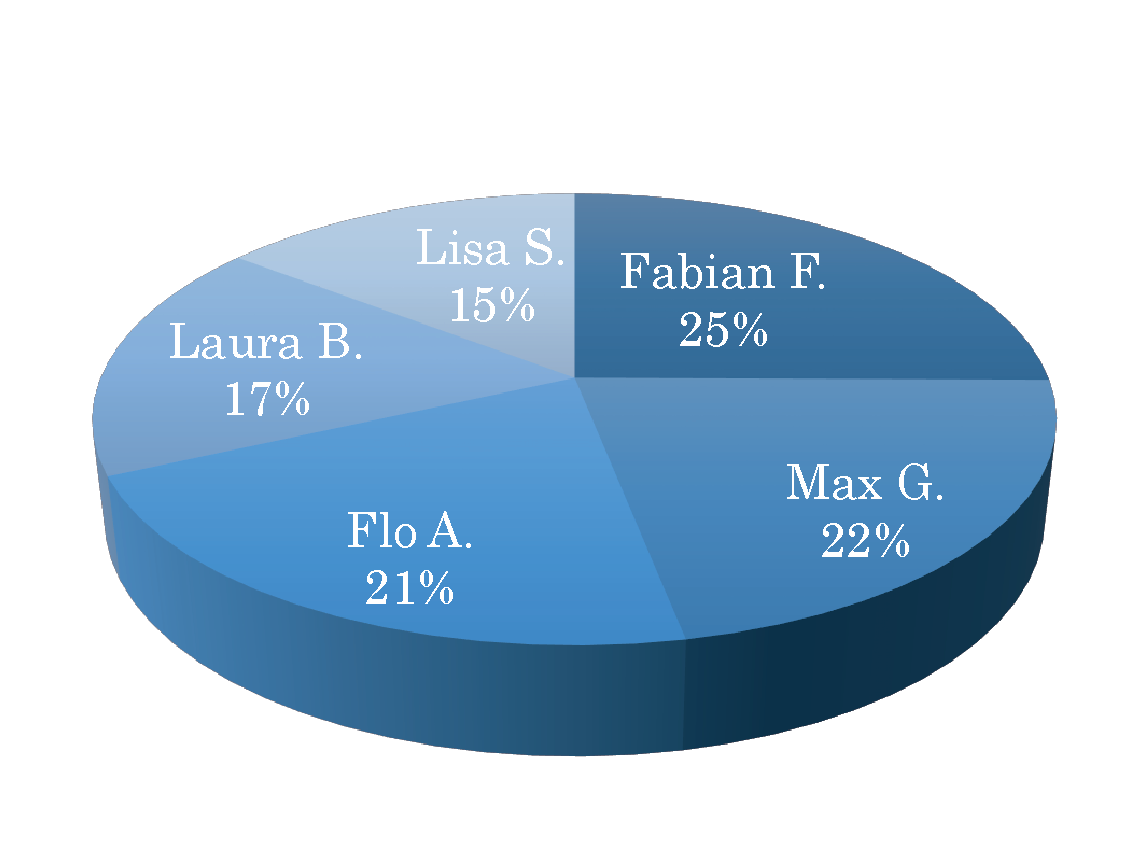
\includegraphics[width=0.49\textwidth]{pics/konzept_tortendiagramm.pdf}}\hfill
\subfigure[Balkendiagramm]{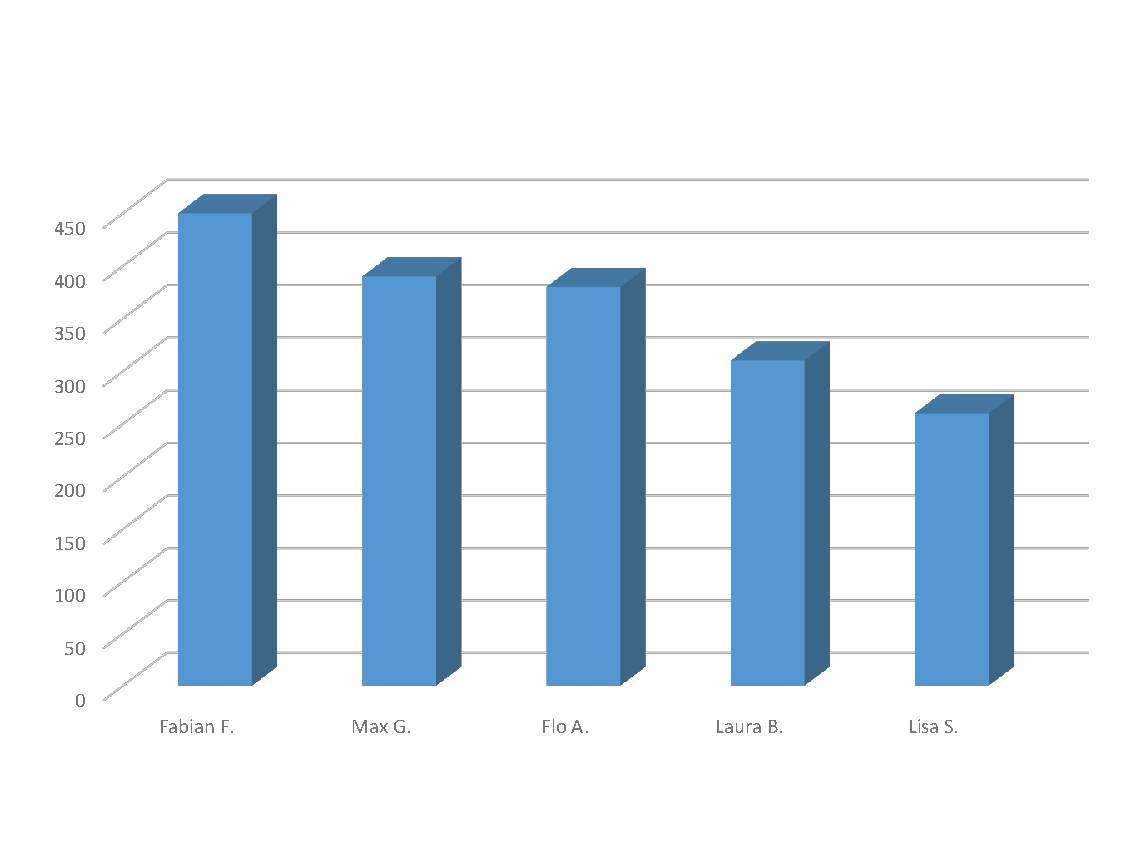
\includegraphics[width=0.49\textwidth]{pics/konzept_balkendiagramm.pdf}}\hfill
\subfigure[Tree Map]{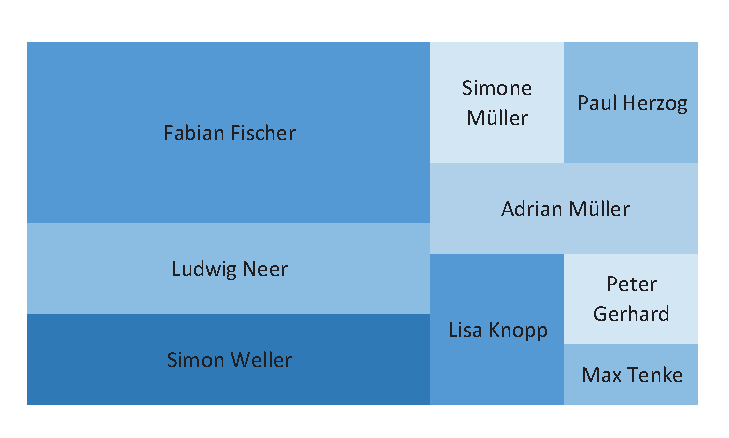
\includegraphics[width=0.49\textwidth]{pics/konzept_tree_map.pdf}}\hfill
\subfigure[Liniendiagramm]{\includegraphics[width=0.49\textwidth]{pics/konzept_liniendiagramm.pdf}}\hfill
\subfigure[Netzdiagramm]{\includegraphics[width=0.49\textwidth]{pics/konzept_netzdiagramm.pdf}}
\caption{Entwürfe für die Oberfläche}
\label{konzept_darstellung}
\end{figure}

Es gibt einige Diagrammtypen allerdings ergeben sich Einschränkungen durch das verwendete Framework. Im Grunde lässt sich jede Darstellung umsetzen, allerdings ist das Aufwand-Nutzen-Verhältnis zu berücksichtigen. In einer Vorauswahl wurden einige  Typen ausgewählt die in Abbildung \ref{konzept_darstellung} (b)-(f) dargestellt sind. 

Netzdiagramme geben Eigenschaften verschiedener Systeme wieder. Sie eignen sich daher gut zur Darstellung von Ausprägungen. Für die vorliegenden Daten ist diese Darstellung gänzlich ungeeignet, da mit Mengen gearbeitet wird. 

Mithilfe von Liniendiagrammen lassen sich Trends und Zeitreihen darstellen. Die Verwendung verschiedener Linien ermöglicht zudem die Darstellung mehrerer Trends. Die Benutzung dieses Diagramms wäre nicht sinnvoll, da die Ergebnismenge sich nicht auf verschiedene Zeitpunkte bezieht, sondern die Summe der Werte aus einer Zeitreihe beinhaltet. 

Bei einer Tree Map steht jede Fläche eines Rechtecks im proportionalen Zusammenhang zur Gesamtfläche. Die Beachtung von Größenverhältnissen stellt eine nützliche Eigenschaft für unsere Daten dar. In unserem Fall würde jedes Rechteck aus dem jeweiligen Anteilen der Verbindungsmerkmale bestehen oder mithilfe eines Drilldowns
\footnote{Als Drilldown wird im Allgemeinen die Navigation in hierarchischen Daten bezeichnet. Auf Oberflächen bezogen wird damit die Darstellung von Detailinformationen durch einem Klick auf Darstellungselemente ausgedrückt.}
 die Verbindungsmerkmale aufzeigen. Beispielweise könnte die Person Ludwig Neer wiederum in Rechtecke unterteilt werden, mit der jeweiligen Anzahl der verschiedenen Verbindungsmerkmale. Das würde allerdings aufgrund zu vieler Kacheln schnell zu einer schlechten Übersicht führen. Wird in einer Tree Map die Drilldown-Navigation gewählt, ist die Übersicht aller Informationen auf einen Blick nicht mehr gegeben. Aufgrund der Nachteile in der jeweiligen Variation wurde sich gegen den Einsatz einer Tree Map entschieden.

Kreisdiagramme ermöglichen eine Betrachtung der Gesamtheit zu ihren Einzelstücken, da der Kreis ein geschlossenes System darstellt. Allerdings müssen alle Teile sich auf die gleiche Basis beziehen. Es eignet sich hervorragend zur Darstellung von Verhältnissen. Wird nun eine weitere Unterteilung der Teilwerte benötigt, geht die Übersicht verloren. Um das zu vermeiden wird die unterteilte Teilmenge häufig in separaten Ansichten dargestellt. Allerdings steigt dadurch der Aufwand für den Nutzer in der Bedienung des Systems. 

Das Balkendiagramm ist für die Darstellung der Daten am geeignetsten. Reihenfolgen beispielsweise lasse sich durch die resultierenden Stufen sehr gut darstellen. Balken selbst lassen sich außerdem in einzelne Teile aufspalten, ohne die Übersichtlichkeit zu verringern. Gegenüber dem Kreisdiagramm kann es zwar keine Betrachtung des Gesamten liefern, allerdings ist das in diesem Anwendungsfall auch nicht nötig. 

%% ===========================
\section{Technologien}
%% ===========================

Als eine der am meist verbreitetsten Programmiersprachen, stellt Java die Grundlage aller verwendeten Technologien dar. Zur Darstellung der Inhalte für den Client wird Vaadin verwendet. Der Apache Tomcat nimmt die Rolle des Anwendungsservers ein. Die Kommunikation auf Basis von RESTful Web Services wird mithilfe von Jersey realisiert. Weiterhin wird opencsv für das Lesen und Schreiben von CSV-Dateien verwendet. JDBC wird zur Kommunikation zwischen dem Anwendungsserver und der Datenbank. Die H2-Datenbank stellt die Datenquelle des Systems dar. Im Folgenden werden alle Bestandteile, bis auf die bereits erläutert H2-Datenbank, näher beschrieben. 

\paragraph{Vaadin}

Vaadin ist ein Open-Source-Framework für den Aufbau von modernen Web-Anwendungen.
Es verwendet ein reines serverseitiges, eventbasiertes Modell und ermöglicht eine Anwendungsentwicklung ohne direkte Verwendung von HTML und JavaScript-Code. Das Framework ermöglicht es, die gesamte Anwendungslogik auf der Serverseite einer Anwendung auszuführen, während die Clientseite nur für das Senden der Benutzeraktionen an den Server und für die Reaktion auf die Antworten verantwortlich ist. Da es auf GWT basiert, kann sowohl der Client- als auch der Server-Code in reinem Java geschrieben werden.

Die aktuelle Version von Vaadin wurde im Februar 2013 veröffentlicht. Die folgenreichste Änderung von Vaadin6 war die Integration von GWT zu Vaadin, die eine bessere Unterstützung für die clientseitige Widget-Entwicklung bedeutet und sogar die Möglichkeit zum Erstellen von Offline-Anwendungen mit sich bringt.

Die im Unternehmen vorhandene Erfahrung und Open-Source stellen relevante Entscheidungsfaktoren in der Wahl von Vaadin. Allerdings war VaadinCharts, eine Erweiterung für Vaadin, für die Auswahl ausschlaggebend. Es basiert auf Highcharts, einem JavaScript-Packet. Highcharts zeichnet sich durch eine umfangreiche Sammlung an Funktionen zur Darstellung von Diagrammen aus. 

\paragraph{Jersey}

Jersey ist ein Open-Source-Framework zur Entwicklung von RESTful Web Services in Java, welches eine Unterstützung für JAX-RS-APIs bietet und die JAX-RS (JSR 311 und JSR 339)-Referenzimplementierung darstellt. JAX-RS-Annotationen werden verwendet um die Relevanz von Java-Klassen für REST zu definieren. Jersey enthält einen REST-Server und einen REST-Client. Auf der Serverseite verwendet Jersey ein Servlet zum Abtasten von vordefinierten Klassen, um REST-Ressourcen zu identifizieren. Über die web.xml Konfigurationsdatei werden die von der Jersey-Distribution bereitgestellten Servlets registriert. Diese Servlets analysieren die eingehenden HTTP-Nachrichten und wählen die richtige Klasse und Methode für die Anfragen aus. Diese Auswahl basiert auf Annotationen in diesen Klassen und Methoden. Weiterhin unterstützt JAX-RS die Erstellung von XML und JSON mithilfe der Java Architektur für XML Binding (JAXB).

\paragraph{Apache Tomcat7}

Tomcat ist ein Open-Source-Webserver, der von der Apache Group entwickelt wurde. Der Apache Tomcat implementiert die Java Servlets-, sowie die JavaServer Pages-Spezifikation von Sun Microsystems und stellt folglich eine Referenzimplementierung dar. Er stellt weiterhin eine rein auf Java-basierende HTTP-Webserverumgebung dar. Weiterhin kann der Tomcat über eine Oberfläche sowie durch Bearbeiten von XML-Dateien konfiguriert werden.

\paragraph{opencsv}

Da Java das Parsen von CSV-Dateien nativ nicht unterstützt, wird auf eine Drittanbieterbibliothek zurückgegriffen. Diese heißt opencsv und ist eine sehr einfache CSV-Parser-Bibliothek für Java. Die Bibliothek kann zum Erstellen, Lesen und Schreiben von CSV-Dateien verwendet werden. Die wichtigste Fähigkeit des opencsv-Parsers ist das Mapping von CSV-Daten auf Java-Bean-Objekte.

\paragraph{JDBC}

Die JDBC-API ermöglicht den programmgesteuerten Zugriff auf relationale Daten, direkt aus der Java Programmiersprache heraus. Durch die Verwendung der JDBC-API können Java-Anwendungen SQL-Anweisungen ausführen, Ergebnisse abrufen und die Veränderungen auf die Datenquelle zurückschreiben. Die JDBC-API kann auch mit mehreren Datenquellen in einer verteilten, heterogenen Umgebung interagieren. 

%% content.tex
%%


%% ===========================
\chapter{Umsetzung}
%% ===========================


%% ===========================
\section{Aufbau der Server.war}
%% ===========================

Das Server Web Archive beinhaltet ein dynamisches Web Projekt aus dem Eclipse Web Tools Platform (WTP) Projekt. Das Project weist die typische Struktur eines Web Projektes auf. Daher wird im folgenden nur auf die Klassen eingegangen. Abbildung \ref{umsetzung_klassendiagramm_server} zeigt das Klassendiagramm der Server.war. Das Diagramm dient als Basis für die nachfolgenden Erläuterungen. 

Die H2-Datenbank wird im Embedded-Modus betrieben, was eine Instanziierung der Datenbank zur Laufzeit notwendig macht. Die Instanziierung erfolgt in der Klasse Database. Das Attribut dataSource stellt die H2-Datenbank in Form eines Objektes dar. Eine Verbindung zur Datenbank wird mithilfe der Methode .getConnection() aufgebaut. Diese Verbindung wird permanent offen gehalten solang der Tomcat Server läuft. Dazu wird die Verbindung dem Attribut con zugewiesen, die von allen Methoden verwendet wird die eine Verbindung zur Datenbank aufbauen wollen. Um die Datenbank mit dem deployen der Web-Anwendungen zu starten, ist die Verwendung eines Servlets nötig. Dazu benutzen wir die Klasse EntryPoint die das Interface HttpServlet implementiert. Um das Servlet direkt beim Start aufzurufen wird in der web.xml folgende Zeilen eingetragen: 

\begin{lstlisting}[language=XML]
	<servlet>
		<servlet-name>H2</servlet-name>
		<servlet-class>de.cas.db.EntryPoint</servlet-class>
		<load-on-startup>1</load-on-startup>
	</servlet>
\end{lstlisting}

Die 1 im Element <load-on-startup> bewirkt den Aufruf der Methode init() die eine Instanziierung der Klasse Database vornimmt. Zur Erzeugung des Schemas wird eine separate Klasse namens SchemaBuilder eingesetzt. In Ihr werden sämtliche SQL-Anweisungen zur Generierung des Schemas aufbewahrt und können über die Methode createSchema() ausgeführt werden.

Mit der Klasse JerseyServer wird der REST-Server umgesetzt. Sie besitzt Methoden die mit dne entsprechenden Annotationen wie @GET oder @OST die REST-Requests entgegen nehmen. Mit der Annotation @Path wird die URL angegeben unter der die Methode angesprochen werden kann. Diese Methoden können Übergabeparameter vom Typ UriInfo und/oder HttpHeaders besitzen, die Abrufe von Metadaten der REST-Requests ermöglichen. 

\begin{figure}[htbp]
\begin{center}
\includegraphics[width=1.0\textwidth]{pics/ServerKlassendiagramm.pdf}
\caption{Server Klassendiagramm}
\label{umsetzung_klassendiagramm_server}
\end{center}
\end{figure}

Neben den Methoden zu Beantwortung von REST-Requests, enthält die Klasse alle Objekte zur Durchführung des ETL-Prozesses. Die Klasse ConnectorJDBC besitzt ein Attribut namens con, welches den Verbindungsaufbau zum MSSQL Server, mithilfe von JDBC ermöglicht. Zur Extraktion der Daten aus dem MSSQL 2008 wird ein Objekt der Klasse QueryBuilder verwendet. Wie in der Abbildung zu sehen, werden für die verschiedenen Tabellen des neuen Schemas, eigene Methoden zur Verfügung gestellt. Methoden welche die Übergabewerte table, date und n besitzen, werden für die verschiedenen Verbindungsobjekte benötigt. Mithilfe des Parameters table, wird der Name der Tabelle in der MSSQL Datenbank übergeben. Der Parameter date gibt das Feld an, was für die Ermittlung des Datums verwendet werden soll. Um den Typ einer Verbindung zwischen Personen festzuhalten, wird der Parameter n verwendet, der eine Zahl zwischen eins und fünf beinhaltet. QueryBuilder verwendet ein Objekt vom Typ CSV-Builder, um die Ergebnisse in Dateien festzuhalten. Den Methoden wird als Übergabeparameter ein Dateiname, sowie die Daten selbst übergeben.

Die Klasse Transform enthält Attribute und Methoden zur Bearbeitung der CSV-Dateien. Weiterhin werden, die durch die Extraktionen gewonnen CSV-Dateien, mithilfe eines CSVReaderWriter Objekts ausgelesen. Nach der Bearbeitung durch die Methoden der Transform-Klasse, werden die Daten wieder in CSV-Dateien abgelegt. CSVBuilder besitzt Methoden die zusätzliche Parameter zum schreiben aufweisen, die modifizierte Schreiboperationen erlauben. Wohingegen CSVReaderWriter mithilfe der Methode writeDataToCSV(), sowie den Parametern path und data allgemeine Schreiboperationen durchführt.

Mithilfe der Klasse Load, wird die Datenbank befüllt. Sie kann wie zuvor erwähnt von einem Database Objekt verwendet werden oder durch ein JerseyServer Objekt. Beim JerseyServer werden mit der Methode load(), die Methoden der Load-Klasse aufgerufen. In der Klasse Database werden sie im Konstruktor aufgerufen. 

Die Logik Klasse enthält alle Attribute und Methoden, zur Beantwortung von Anfragen, durch den Nutzer. Zur Generierung der Bedingungen einer SQL-Abfrage, werden separate Methoden verwendet. Die jeweiligen Methoden werden nur gerufen, sobald die entsprechende Bedingung, in der vom Nutzer erhaltenen JSON Datei, vorhanden ist. Angesteuert wird der Bau einer Abfrage durch die Methode buildQuery(). 

%% ===========================
\section{Aufbau der Client.war}
\label{ch:Umsetzung:sec:clientwar}
%% ===========================

\begin{figure}[htbp]
\begin{center}
\includegraphics[width=1.0\textwidth]{pics/ClientKlassendiagramm.pdf}
\caption{Client Klassendiagramm}
\label{umsetzung_klassendiagramm_client}
\end{center}
\end{figure}

Einstiegspunkt in der Client.war ist die Klasse CasAnalyticUI. Sie ist von der Klasse UI abgeleitet. Die UI ist die oberste Komponente jeder Komponentenhierarchie. Es gibt eine Benutzeroberfläche für jede Vaadin-Instanz in einem Browser-Fenster. Ein UI Objekt kann entweder ein gesamtes Browser-Fenster (oder Tab) oder einen Teil einer HTML-Seite, wo eine Vaadin-Anwendung eingebettet ist, darstellen. Nachdem eine UI von der Anwendung erstellt wurde, wird es mit der Methode init(VaadinRequest) initialisiert. Zur Übersicht werden die Komponenten der Darstellung in die Klasse RootUI ausgelagert. 

RootUI wird dabei von der CasAnalayticUI instanziiert. Die Klasse RootUI beinhaltet das Anmeldefenster, sowie die Hauptansicht. Mithilfe der Methode buildLoginView() werden die Komponenten des Anmeldefensters zur UI hinzugefügt. Nach der Erzeugung der Komponenten, wird eine JerseyClient Klasse instanziiert. Diese wird verwendet sobald der Nutzer IP, Port und einen Namen eingegeben hat und auf anmelden geklickt hat. Anschließend wird die Methode doPostRequestUserData() gerufen, um zu überprüfen ob der Nutzer im System existiert. 

Falls ja werden durch die Methode MainView() alle bisherigen Komponenten der UI entfernt und durch Komponenten des Hauptfensters ersetzt. Das JerseyClient Objekt wird direkt im Anschluss verwendet, um Mithilfe der Methode doPostRequestData() einen REST-Request an den Server zu senden. Dieser liefert das Ergebnis der Abfrage in einem JSON-Objekt zurück. Mit dessen eine erste Darstellung der Diagramms erzeugt wird. Das Diagramm selbst besitzt eine eigene Klasse namens ChartComponent. Sie leitet sich von der Klasse Chart ab, die Teil der VaadinChart Bibliothek ist. Mithilfe der Methode refreshChart() wird das Diagramm bei Benutzerabfragen aktualisiert. Dazu werden ihr die Namen der Personen für die x-Achse übergeben, sowie die neuen Balkenwerte. Weiterhin wird für jedes Vaadin-Objekt das eine Element an der Oberfläche darstellt, eine separate Methode zur Erzeugung verwendet. Änderungen am Aussehen oder der Funktion, der jeweiligen Vaadin-Objekte, werden nur innerhalb der entsprechenden Methode vorgenommen.

An der Oberfläche gibt es Felder die nur Zahlen erwarten. Eingaben die nicht numerisch sind, werden durch den Einsatz der Klasse IntegerField verhindert. Diese erweitert die Klasse TextField. Sie besitzt einen Event-Listener, der jede Eingabe des Benutzers abfängt. Gibt der Nutzer nicht numerische Zeichen ein werden diese direkt wieder entfernt. Dadurch werden falsch Eingaben durch den Nutzer ausgeschlossen.

%% ===========================
\section{Erzeugung der Abfrage}
%% ===========================

Um Abfragen durch den Benutzer möglichst performant zu beantworten erfolgt die Erzeugung dynamisch. Das bedeutet die SQL-Abfrage an die Datenbank kann je nach Anforderung anders aufgebaut sein. Die Kernaufgabe ändert sich jedoch nie. Diese besteht aus der Bildung von Summen basierend auf verschiedenen Verbindungstypen. Zu Berücksichtigen ist das jede Abfrage einen Anfangs- und Endzeitpunkt enthält und somit beachtet werden muss. Nachdem festgestellt wurde wie viele Verbindungen von den jeweiligen Typen zu einer Person verlaufen wird zusätzlich die Gesamtsumme der Verbindungen zu einer Person gebildet. Die Summe wird zur Sortierung der Ergebnisse verwendet. Bei der Sortierung wird absteigend vorgegangen um die Personen mit den meisten Verbindungen zu der von der Suche ausgehend Person zu ermitteln. Das Ergebnis wird wiederum auf eine durch den Benutzer festgelegte Anzahl reduziert. 

Zu diesen Kernfunktionalitäten können durch Angaben des Nutzers weitere hinzukommen. Eine von Ihnen ist die Gewichtung von Zeitpunkten. Der Ansatz zur Umsetzung der Gewichtung der Zeit wird anhand der Abbildung \ref{fig:umsetzung:gewichtungderzeit} erklärt. Die Abbildung zeigt ein Koordinatensystem mit den Gewichtung von einzelnen Zeitpunkten. Die x-Achse stellt den zeitlichen Verlauf dar. Während die y-Achse die Gewichtung darstellt. $t_{start}$ markiert den Startzeitpunkt, wohingegen $t_{end}$ den Endzeitpunkt angibt. Mithilfe von $t_1$ und $t_2$ werden Zeitspannen festgelegt, die differenziert zu gewichten sind. Um nun die Tage zu gewichten wurde der lineare Ansatz gewählt. Das bedeutet zwischen $t_{start}$ und $t_1$ steigt die Relevanz stetig bis sie die 100 Prozent erreicht hat. Ab dort sind alle Tage wieder 100 Prozent relevant außer es ist ein $t_2$ angegeben worden. Falls ja wird ab $t_2$ linear fallend, jeder Tag bewertet. 

Zur Berechnung der Gewichtung zu einem bestimmten Tag werden die folgenden zwei Variablen verwenden:

\begin{equation}
f_1 = \frac{1}{t_1 - t_{start}}
\end{equation}
\begin{equation}
f_2 = \frac{1}{t_{end} - t_2}
\end{equation}

Dabei wird wie folgt vorgegangen. $t_{start}$ markiert Tag. Aufsteigend zählend wird jeder Tag bis $t_1$ mit der Variabel $f_1$ multipliziert. Für den Zeitpunkt $t_2$ wird die Summe der Tage in der Zeitspanne zwischen $t_2$ und $t_{end}$ verwendet. Die Summe wird mit jedem weiteren Tag um 1 vermindert bis zum Zeitpunkt $t_{end}$, der 0 darstellt. Bei jedem Schritt wird der Tag mit der Variablen $f_2$ multipliziert.

\begin{figure}[htbp]
\begin{center}
\begin{tikzpicture}[domain=-1:2] \draw[very thin,color=gray] (0,0); 
\draw[->] (0,0) -- (12.3,0) node[right] {Zeit}; 
\draw[->] (0,0) -- (0,4.2) node[above] {Faktor Gewichtung}; 
\draw[color=black]  (0.2,3) -- (-0.2,3)   node[left] {100\%};
\draw[color=black]  (0.2,1.5) -- (-0.2,1.5)   node[left] {50\%};  
\draw[dashed][color=black]  (5,0.5) -- (5,3.5); 
\draw[dashed][color=black]  (9,0.5) -- (9,3.5);

\draw[color=black]  (0,0) -- (0,0)   node[below] {$t_{start}$}; 
\draw[color=black]  (5,0.1) -- (5,-0.1)   node[below] {$t_1$}; 
\draw[color=black]  (9,0.1) -- (9,-0.1)   node[below] {$t_2$};
\draw[color=black]  (12,0.1) -- (12,-0.1)   node[below] {$t_{end}$};   
 
\draw[color=black]  (0,0) -- (5,3)   node[right] {}; 
\draw[color=black]  (5,3) -- (9,3)   node[right] {}; 
\draw[color=black]  (9,3) -- (12,0)   node[right] {};  

\end{tikzpicture} 
\end{center}
\caption{Gewichtung der Zeit}
\label{fig:umsetzung:gewichtungderzeit}
\end{figure}

Neben der Gewichtung der Zeit lassen sich die jeweiligen Verbindungstypen unterschiedlich gewichten. Bei einer Abweichung von 100 Prozent wird die Summe des jeweiligen Verbindungstypen um die durch den Nutzer bestimmten Prozentsatz verringert. 

Die restlichen Parameter dienen der Filterungen und werden je nach Nutzer-Eingabe zu den Bedingungen der SQL-Abfrage hinzugenommen. Unter Ihnen gibt es eine Bedingung zuvor Ermittelt werden muss und daher näher beschrieben wird. Dabei handelt es sich um das ausschließen von Gruppen, da sich Ihre Zusammensetzung über die Zeit variabel ist. Dazu wird die Tabelle UserGroup verwendet. Dabei wird wie folgendermaßen vorgegangen. Zuerst wird die Ergebnismenge auf die ausgewählten Gruppen reduziert. Anschließend wird für jede Gruppe ein eigener Container erzeugt, der alle Personen der Gruppe enthält. Liegt nun das Feld Date nach dem Anfangszeitpunkt der Abfrage und die Spalte Action enthält eine 1, wird der Container um diese Person reduziert. Enthält die Spalte Action eine 0 wird die Person zum Container hinzugefügt. Die 1 in der Spalte Action bedeutet das die Person zu dem in der Spalte Date angegeben Datum die Gruppe verlassen hat. Eine 0 bedeutet das die Person zu dem angegeben Datum hinzukam. Dadurch wird die Zusammensetzung zum Anfangszeitpunkt wiederhergestellt. Mithilfe der Personen aus den Container wird nun die SQL-Abfrage um weitere Bedingungen erweitert.

Zu beachten ist natürlich das innerhalb des Zeitraums Gruppenveränderungen stattgefunden haben können, diese jedoch nicht zu Berücksichtigen sind. Es kann jeweils nur ein bestimmter Zeitpunkt für die Betrachtung berücksichtigt werden. In diesem Fall wurde der Anfangszeitpunkt gewählt.

%% ===========================
\section{ETL Prozess}
%% ===========================

Um an die notwendigen Daten zu gelangen werden zuerst die Informationen aus der alten Datenbank extrahiert. Dazu wird ein Verbund gebildet der die Tupeln der Tabellen verschmelzen lässt. Die manuellen erstellten Verbindungen in der alten Datenbank werden mithilfe der Tabelle TableRelation festgehalten. Zur Gewinnung dieser Verbindungen wird als erstes eine SQL-Abfrage definiert die für jede der Tabellen gwOpportunity, gwPhoneCall0, Document0, EmailStore0 und Appointment0 separat ausgeführt wird. 

Mithilfe des ersten Verbundes zwischen SysUser und Adresse wird die Adresse einer Person ermittelt. Anschließend wird durch einen Verbund der TableRelation und SysUser alle Tabellen ermittelt die mit der Person eine Verbindung besitzen. Der nächste Verbund ist zwischen TableRealtion und einer der fünf zuvor genannten Tabellen. Um festzustellen welche Personen auch mit beispielsweise einem Dokument arbeiten zu ermitteln wird ein weiterer Verbund mit der passenden ORel-Tabelle ausgeführt. In der ORel-Tabelle kann die OID positiv sowie negativ sein. Bei einem negativen Wert stellt die OID eine GID der Tabelle SysGroup dar. Zur Auflösung der Gruppe in einzelne Personen werden folgende Verbunde gebildet. Zuerst zwischen SysGroup und SysGroupMember um alle Personen die zu einer Gruppe gehören zu erhalten. Anschließend zwischen SysGroupMember und SysUser um die OID der Person zu erhalten. 

Nachdem alle Information in einem Verbund vorhanden sind werden lediglich drei Informationen des Gesamten Verbundes behalten. Zu einem die OID des SysUser von dem die Suche ausgeht. Zum anderen das Datum welches durch das Objekt welches die Personen verbindet ermittelt wird. Weiterhin wird die zweite OID durch den Verbund mit einer zweiten SysUser Tabelle behalten. Zum Schluss wird manuell eine vierte Information beigefügt die besagt welchem Objekt die Tupel entstammt. 

Für den Sonderfall das ein Datum über mehrere Tage geht wird eine fünfte Spalte hinzugefügt welche den Zeitraum in Tagen beinhaltet. Zur Beschaffung der geschobenen Termine wird genau wie in der Konzeption beschrieben verfahren.

Zur Ermittlung direkter Verbindungen zwischen Personen wird lediglich ein Verbund aus zwei ORel-Tabellen eines Objektes gebildet. Dieser Verbund beinhaltet bereits die OIDs der beiden Personen. Zur Ermittlung des Datums wird noch ein Verbund mit der Tabelle des Objektes gebildet. Die negativen OIDs werden genauso wie oben beschrieben aufgelöst. 

Jede Antwort einer SQL-Abfrage zur Gewinnung von Daten wird in einer SCV-Datei direkt auf dem Tomcat Server abgelegt. Diese CSV Dateien stellen die Grundlage der Transformation dar. Jede dieser Dateien beinhaltet Verbindungen zwischen Personen in der Form wie sie Abbildung \ref{fig:umsetzung_csv_datei} zeigt. 

\begin{figure}[htbp]
\begin{center}
\includegraphics[width=1.0\textwidth]{pics/umsetzung_csv_datei.png}
\caption{Ausschnitt einer CSV-Datei mit Daten der Extraktion}
\label{fig:umsetzung_csv_datei}
\end{center}
\end{figure}

Alle CSV-Dateien werden auf die in Abbildung \ref{fig:umsetzung_csv_datei} zu sehenden Ungereimtheiten untersucht. Dabei werden Zeilen wo die letzten fünf Werte fehlen über die die OID (die vierte Zahl) die Adresse ergänzt. Bei null Werten wird überprüft ob wirklich keine Adresse vorhanden ist falls doch werden diese ebenfalls ergänzt. Wenn wie in Zeile 1707 zu sehen eine null Anstatt einem Datum steht wird die Zeile entfernt. Falls wie in Zeile 1708 ein zusätzlicher zehnter Wert vorhanden ist, bedeutet das die Verbindung über mehrere Tage geht. Die Zeile bleibt bestehen jedoch wird der letzte Wert entfernt. Die Zahl wird jedoch noch verwendet um die weiteren Zeilen mit aufsteigendem Datum zu erzeugen. Nach der Beseitigung von Anomalien werden noch die Städte und Länder durch ihre jeweilige ID aus der Tabelle Town und Country ersetzt.

Die veränderten Daten werden wieder in CSV-Dateien abgelegt die gleich bezeichnet sind allerdings noch den Zusatz "\_transf" besitzen der Sie als Transformiert  markiert. Diese Dateien werden anschließend in eine CSV-Datei zusammengeführt. Bei der Zusammenführung sind zum ersten mal alle Daten gleichzeitig in der Anwendung weshalb an dieser Stelle alle Duplikate beseitigt werden. Weiterhin werden die Zeilen sortiert. Dabei wird mit zwei Kriterien sortiert. Das erste Kriterium ist der Erste Wert die OID der Person von dem die Suche ausgeht. Wenn hierbei gleiche Werte verglichen werden wird das zweite Feld(Datum) herangezogen. Nachdem alle Zeilen sortiert und von Duplikaten bereinigt sind werden alle Zeilen in einer CSV-Datei abgelegt. 

Diese Datei wird bei jedem Start des Tomcats dazu verwendet einen Bulk-Load für die H2-Datenbank zu initialisieren. Nachdem die Datenbank mit Daten befüllt wurde werden abschließend die Indizes erzeugt.


%% ===========================
\section{Aktualisierung des Datenbestandes}
%% ===========================

%% ===========================
\section{Oberfläche}
%% ===========================

In diesem Abschnitt wird die Umsetzung auf der Darstellungsebene erörtert. Den Einstiegspunkt für Nutzer stellt das in Abbildung \ref{ergebniss_oberflaeche_anmeld} zu sehende Anmeldefenster dar. Der Hintergrund der Webseite ist in einem dunklen grau Gestaltet, um sich von dem weißen Hintergrund der Bedienelemente abzuheben. Zur Identifikation des Systems mit der Firma ist dessen Logo im linken Teil dargestellt. Im rechten Teil des Fensters existieren drei Eingabefelder. Zuerst ein Feld zur Eingabe der IP-Adresse des Server. Die dazugehörige Portnummer wird im darauf folgenden Feld eingegeben. Das dritte Feld ist für den Namen des Nutzers vorgesehen, der den Ausgangspunkt der Analyse darstellt. Abschließend wird ganz klassisch ein Button zum fortfahren auf der Webseite eingesetzt. Falls allerdings der eingegeben Nutzername nicht existiert wird eine Warnmeldung direkt über dem dafür vorgesehen Feld ausgegeben. 

\begin{figure}[htbp]
\centering
\includegraphics[scale=2.0]{pics/login.png}
\caption{Oberfläche des Systems}
\label{ergebniss_oberflaeche_anmeld}
\end{figure}

Das Hauptfenster wurde vom Aufbau wie in Abschnitt \ref{ch:Konzeption:sec:Darstellungskonzepte} beschrieben umgesetzt. Im oberen Bereich findet sich eine Leiste, die an Produkte wie Microsoft Office angelegt ist. Dies schafft ein vertrautes Gefühl mit der Oberfläche, da auf bekanntem aufgebaut werden kann. Die Leiste ist in vier Bereiche gegliedert. Der erste Bereich, ganz links, dient der Gewichtung von Suchkriterien und der Anfragestellung. Aufgrund der Gewichtung in Prozent ist ein fester Wertebereich von 0 bis 100 vorgegeben. Textfelder eignen sich daher weniger, da sie beliebige Eingaben ermöglichen. Der Einsatz von Reglern bietet eine einfachere und selbsterklärende Form der Bedienung. Der begrenzte sowie kleine Wertebereich führten zu der Entscheidung. Zum stellen der Anfrage wird ein einfacher Button eingesetzt. Direkt unter dem Button befindet sich Text, der zur Ausgabe der benötigten Zeit vorgesehen ist. 

Der zweite Bereich in der Mitte dient zeitlichen Anpassungen. Das erste und dritte Feld können zur Veränderung der Zeitspanne verwendet werden. Sie beinhalten den Anfangs- und Endzeitpunkt der Betrachtung. Händische Eingaben sind eher schlecht für die Bedienbarkeit weswegen ein sogenannter Datumspicker eingesetzt wird. Dieser befindet sich direkt neben dem Textfeld und öffnet sich nach einem klick auf das Symbol. Er stellt einen grafischen Kalender dar aus dem durch klicken auf ein Tag das Datum bestimmt werden kann. Die Möglichkeit zur Eingabe durch direktes ändern des Textes bleibt allerdings weiterhin erhalten. Die anderen beiden Felder sind für die Gewichtung der Zeit vorgesehen. In Abbildung \ref{fig:umsetzung:gewichtungderzeit} werden die Zeitpunkt bis zu dem differenziert gewichtet werden soll mit $t_1$ und $t_2$ bezeichnet. Diese Zeitpunkte können mithilfe der Textfelder bestimmt werden. Das obere Feld ist für $t_1$. Hier kann die Zeitspanne zwischen $t_{start}$ und $t_1$ in Tagen festgelegt werden. Für $t_{ende}$ und $t_2$ verhehlt es sich mit dem unteren Feld ebenso.

Bis auf die Gruppenfilterung sind im dritten Bereich alle restlichen Filtermöglichkeiten vorhanden. Mithilfe von Checkboxen kann der Nutzer festlegen welche Filterungen auf die Analyse angewendet werden sollten. Neben der Filterung durch bestimmte Personen, Länder, Städte usw. ist hier eine Begrenzung der Ergebnismenge umgesetzt. Im untersten Feld kann der Nutzer diese bestimmen.

Der Bereich ganz rechts in der Leiste ist für den Ausschluss von Gruppen vorgesehen. Hier werden alle Gruppen im System mit einer Checkbox und einem Namen dargestellt. Dabei können beliebig viele Gruppen ausgewählt werden. Da die Anzahl der Gruppen überschaubar ist entschied man sich alle anzuzeigen anstatt einer manuellen Eingabe durch den Nutzer. Das hat auch den Vorteil, dass der Benutzer Gruppen sieht die er eventuell nicht exakt beim Namen kennt.     

\begin{figure}[htbp]
\centering
\includegraphics[width=\textwidth]{pics/final_screen.png}
\caption{Oberfläche des Systems}
\label{ergebniss_oberflaeche_haupt}
\end{figure}

Den zentrale Bereich des Fensters stellt das Diagramm dar. Die Balken selbst sind fünf verschiedene Elemente unterteilt. Jedes Elemente wird dabei durch eine andere Farbe dargestellt. Die fünf Elemente sind die verschiedenen Merkmale. Die Zuordnung der Farbe zu dem jeweiligen Merkmal wird über eine Legende im unteren Bereich des Fensters umgesetzt. Eine Besonderheit ist, dass durch einen Klick auf eine der Farben, das jeweilige Merkmal von der Darstellung ausgeschlossen wird. Beispielsweise kann der Nutzer auf die blaue Farbe neben dem Dokument klicken, was einen Neuaufbau des Diagramms, ohne dieses Merkmal bewirkt. Durch diesen Ausschluss wird allerdings keine neue Abfrage gesendet. Das  bedeutet die Reihenfolge in der Personen angezeigt werden bleibt gleich, sowie die Datenbasis. Mit einem wiederholten Klick lässt sich das ganze Rückganggig machen. Zusätzlich zu der Y-Achse, die eine Gesamtpunktzahl aufzeigt, kann der jeweilige Anteil eines Merkmals betrachtet werden. Dies geschieht durch einfaches platzieren des Mauszeigers auf dem jeweiligen Bereich des Balkens. Dadurch öffnet sich ein Tooltip welches die Anzahl der Punkte im Verhältnis zur Gesamtpunktzahl zeigt.

Die Anfragestellung erfolgt in der Regel mit dem dafür vorgesehen Button. Die Regler und das Datum lösen jedoch bei Veränderungen automatisch eine neue Abfrage aus. Dies soll die  die hohe Antwortgeschwindigkeit des Systems untermalen. Das Datum sowie die Gewichtung wurden dafür ausgewählt da diese die am meist benutzen Konfigurationsmöglichkeiten darstellen.
%% Cahpter_Zusammenfassung.tex
%%

%% ===========================
\chapter{Fazit und Ausblick}
\label{ch:Ergebnis}
%% ===========================

In diesem abschließenden Kapitel werden die Ergebnisse dieser Arbeit in ihren wichtigsten Punkten zusammengefasst und anhand der Anforderungen aus Kapitel \ref{ch:Systemanalyse:sec:Anforderungsanalyse} bewertet. Anschließend wird ein Ausblick auf weiterführende Möglichkeiten, sowie zukünftige Verbesserungsmöglichkeiten gegeben. 

%% ===========================
\section{Zusammenfassung}
\label{ch:Ergebnis:sec:zusammenfassung}
%% ===========================

Aus der Motivation heraus wurde in der vorliegenden Arbeit, ein analytisches System, basierend auf den CAS genesisWorld Daten entwickelt. Hierzu wurden zuerst alle relevanten, operativen Komponenten für die Entwicklung ermittelt. Anschließend wurde eine Szenario festgelegt, in dessen die Personen ausgeprägtesten Beziehung, zu einer ausgewählten Person ermittelt werden sollte. Mit dieser Frage im Hinterkopf, wurde die Datenbank nach den passenden Datensätzen, zur Beantwortung der Aufgabenstellung durchsucht. Nachdem klar war, welche Daten zu übernehmen sind, wurde eine passende Datenbank ausgewählt. Diese sollte den zuvor erhobenen Anforderungen gerecht werden. Dabei wurden NoSQL-Datenbanken hinsichtlich ihrer Eignung untersucht. Sie konnten in diesem Fall allerdings nicht überzeugen, somit entschied man sich für die H2-Datenbank. Die durch ihre im Hauptspeicher gehaltenen Tabellen überzeugen konnte.   

Aufbauend auf der bereits getätigten Wahl der Datenbank, wurden Konzepte zur Umsetzung des Systems entwickelt. Bei der Konzeption wurde deduktiv vorgegangen. Zuerst wurde die Architektur festgelegt. Aufbauend auf ihr wurden die einzelnen Komponenten detailliert geplant. Bei der Planung wurde nicht versucht ein universell einsetzbares System zu entwickeln, sondern vielmehr eine domänenspezifische Lösung für das Szenario zu erreichen. Nachdem alle Technologien, sowie Vorgehensweisen festgelegt wurden, ging man auf die Umsetzungen ein. Indessen eine Beschreibung der Funktionsweisen der einzelnen Komponenten durchgeführt wurde. Neben der Funktionsweise wurden die Interaktion unter den Komponenten dargelegt. Schließlich ging man noch auf die Umsetzung der Darstellung ein und den damit verbundenen Designentscheidungen ein. 
 
%% ===========================
\section{Bewertung der Ergebnisse}
\label{ch:Ergebnis:sec:bewertung}
%% ===========================

Die funktionalen Anforderungen konnten alle umgesetzt werden und wurden bereits im vorherigen Kapitel erläutert. Im folgenden wird somit auf die Erfüllung der nicht funktionalen Anforderungen eingegangen. Dies erfolgt anhand der Gegenüberstellung von Anforderungen und den Charakteristika des Systems.

Die erste Anforderung die eher eine Rahmenbedingung darstellt, konnte eingehalten werden. Zur Umsetzung der Lösung wurde ein einziger Server verwendet. Weiterhin wurde eine lose Kopplung erreicht. Dies spiegelt sich in den REST-Schnittstellen, der jeweiligen Komponenten wieder. Überdies gibt es keine Abhängigkeiten zwischen den Klassen der Darstellung und den Klassen der Geschäftslogik. Ein gewisses Maß an Portabilität wurde vorausgesetzt, damit ein verlagern des Systems auf andere Instanzen kein problem darstellt. Dies wurde durch die Verwendung der Web-Archive-Dateien erreicht. Sie ermöglichen den Einsatz auf verschiedenen Tomcat Servern, was sie nicht nur portabel macht, sondern auch noch dessen Einsatz auf verschiedenen Servern erlaubt. 

Einer der wichtigsten Anforderungen ist die geringe Abfragegeschwindigkeit. Tabelle \ref{tb:vergleichAbfragegeschwindigkeit} zeigt, dass man dieser Forderung gerecht wird. Ebenfalls deutlich zu erkennen, ist die Auswirkung des geänderten Schemas. Der Sprung von 98.000 ms auf 350 ms, ist durch die Reduktion der Abfragekomplexität zu erklären. Im neuen Schema existieren weniger Tabellen und Tupeln. Außerdem ist im neuen Schema kein Verbund in der Datenbankabfrage mehr notwendig, der sehr rechenintensiv sein kann. Allerdings ist zu beachten, dass solche Maßnahmen, wie sie im Schemadesign ergriffen wurden weitreichende Folgen haben. Eine davon ist eine sehr schlechte Erweiterbarkeit des Schemas. Im momentanen Schema können lediglich Spalten hinzugezogen werden, dessen Inhalt in allen Verbindungsmerkmalen vorhanden ist. Außerdem würde für jede Spalte weitere 18 Mio. Werte hinzukommen. Die Hinzunahme von merkmalspezifischen Attributen führt ebenfalls zu hohen Änderungsaufwänden. Die Konsequenz die daraus gezogen werden müsste, wäre eine stärke Normalisierung des Schemas, die die \textit{data} Tabelle in mehrere Tabellen aufteilen würde. Dies würde wiederum den Einsatz von Verbundoperatoren erfordern. Dadurch würde die Abfragezeit wieder steigen. Allerdings wären wesentlich weniger Verbundoperatoren nötig als im alten Schema. Aufgrund dessen ist trotzdem mit einer deutlichen geringeren Abfragegeschwindigkeit als in CAS genesisWorld zu rechnen.  

\begin{table}[htbp]
\centering
\begin{tabular} {l | r}
Versuchskomponente & Zeit in ms  \\ \hline
MSSQL Datenbank \& Altes Schema & 98000 \\
MSSQL Datenbank \& Neues Schema & 350 \\
H2 Datenbank \& Neues Schema & 80 \\
\end{tabular}
\caption{Abfragegeschwindigkeit Vergleich}
\label{tb:vergleichAbfragegeschwindigkeit}
\end{table}

Bei Änderungen die eine Steigerung der Komplexität mit sich bringen, stellt sich eine Frage. Ist die Datenbank nur aufgrund des geänderten Schemas deutlich schneller? Um dieser Frage nachzugehen wurden einige Tests durchgeführt. Abbildung \ref{ergebniss_vergleich} zeigt die Ergebnisse dieser Testreihen. Alle Test wurden auf einem Rechner durchgeführt. Dieser simulierte den Zugriff von 100 gleichzeitigen Benutzern, mithilfe von Multithreading. Die in den Diagrammen angegebene Zeit bezieht sich somit auf die Ausführung aller 100 Abfragen. Jeder simulierte Benutzer führt somit, die auf der y Achse angegebene Anweisung aus. Beim obersten Balken in (a) sind es beispielsweise 15 Mio. SELECT-Anweisungen pro Benutzer. In (b) hingegen wird die Verarbeitungsgeschwindigkeit bei Updates verglichen. Der Vergleich anhand von Insert-Anweisungen wird in (c] gezeigt.    

\begin{figure}[htbp]
\centering
\subfigure[Vergleich anhand Select-Performance]{\includegraphics[width=0.49\textwidth]{charts/select.pdf}}\hfill
\subfigure[Vergleich anhand Update-Performance]{\includegraphics[width=0.49\textwidth]{charts/update.pdf}}\hfill
\subfigure[Vergleich anhand Insert-Performance]{\includegraphics[width=0.5\textwidth]{charts/insert.pdf}}
\caption{Abfragegeschwindigkeit Vergleich}
\label{ergebniss_vergleich}
\end{figure}

Die Ergebnisse der Tests zeigen, dass die H2-Datenbank bei den durchgeführten Tests deutlich schneller als die MSSQL Datenbank ist. Der H2 ist bei SELECT-Anweisungen, um den Faktor 37 schneller. Bei Update-Anweisungen sogar um den Faktor 117. Ebenso bei Insert-Anweisungen, die einen Unterschied um den Faktor 124 aufweisen. Daraus lässt sich ableiten, dass die H2-Datenbank durch ihre In-Memory-Tabellen deutlich an Geschwindigkeit, im Gegensatz zu herkömmlichen Datenbanken, gewinnt. Diese Geschwindigkeit wird zum Teil durch den Verzicht auf Persistenz erlangt. Zum anderen durch die Nutzung des Hauptspeichers als Speichermedium. Im vorliegenden System, welches fast nur Leseoperationen durchführt, stellt die mangelnde Persistenz allerdings kein großes Defizit dar. Die Nutzung des Hauptspeicher könnte allerdings in der Zukunft, aufgrund der immer größer werdenden Datenmengen, ein Problem darstellen.  

%% ===========================
\section{Ausblick}
\label{ch:Ergebnis:sec:Ausblick}
%% ===========================

Mit der Umsetzung des in der Arbeit beschriebenen Systems steht eine eine performante Lösung bereit, die Untersuchung und Bewertung von Beziehungen zwischen Personen ermöglicht.

Die Bewertung der Beziehungen beruht derzeit lediglich auf der Anzahl von Verbindungsmerkmalen. Dabei wird nur die Häufigkeit gewertet. Um die Ausprägung einer Beziehung noch genauer feststellen zu können, werden zusätzliche Regeln benötigt. Diese Regeln müssten auf psychologischen Erkenntnissen und Erfahrungswerten aufbauen. Durch Regeln könnte die Aussagekraft von Ergebnissen weiter steigen. Beispielsweise ist die Kommunikation durch Termine, Telefonate und E-Mail Verkehr, kein Indikator für Vertrauen oder dergleichen. Dokumente in die man anderen Personen Einsicht gewährt und nicht öffentlich sind, setzen eine engere Zusammenarbeit oder Vertrauen voraus. Dies sollte somit stärker gewichtet sein als beispielsweise ein Telefonat. Neben den festen Regeln sind Vorschläge für die Benutzer über verschiedenen Gewichtung der Verbindungsmerkmale sinnvoll. Dabei kann der Nutzer zwischen verschiedenen Vorgaben wählen, die basierend auf Erkenntnissen und Erfahrungen beruhen. Jeder dieser Vorschläge verkörpert verschiedene Charakteristiken. Beispielsweise könnte eine solche Vorgabe wie folgt aussehen. Telefonate, E-Mail und Termine könnten viel stärker gewichtet werden, falls Interesse besteht zu erfahren mit welchen Personen am meisten direkter Kontakt besteht. Diese Einstellungen zur differenzierten Gewichtung zwischen den Verbindungsmerkmalen, könnten als vordefinierte Regeln angeboten werden.

Weiterhin kann durch den Einsatz des Systems, der Vertrieb eines Unternehmens unterstützt werden. Eines der denkbaren Szenarien setzt eine Erweiterung des Systems voraus. Mithilfe von zusätzlichen Informationen über den Wert der jeweiligen Person für die Firma, könnten Vergleiche angestellt werden. Diese Vergleiche könnten anhand von Abgleichen der Position des Kunden im Ranking der Beziehung und dem Ranking anhand des Wertes eines Kunden erfolgen. So könnte Unstimmigkeiten in Aufwand und Nutzen entdeckt werden.
Außerdem könnte jeder Vertriebsmitarbeiter mithilfe des Systems eine individuelle Unterstützung erfahren. Hierbei könnte das Ranking, der Personen mit den stärksten Beziehungen zum Vertriebsmitarbeiter herangezogen werden. Dadurch können Vertriebsmitarbeiter überprüfen ob sie dem jeweiligen Kunden genug Zeit widmen oder anderen zu wenig. Auch könnte das Ranking durch eine sehr simple Manipulation so geändert werden, dass die Personen angezeigt werden mit denen man am wenigsten zu tun hat. Was wiederum eine Überprüfung auf mangelhafte Kundenpflege ermöglicht. 
Überdies könnten Möglichkeiten zum Vergleich mehrerer Personen realisiert werden. Der Vergleich könnte dabei unter Personen aus einer Gruppe oder aus einer durch den Nutzer zusammengestellten Menge erfolgen. Mithilfe eines Vergleichs unter Vertriebsmitarbeitern könnte überprüft werden, ob die Verteilung der Kunden auf einzelne Mitarbeiter effizient gestaltet ist. Beispielsweise läse sich damit feststellen ob zu viele Mitarbeiter sich unwissentlich auf einen Kunden konzentrieren.
Eine weitere weiterführende Möglichkeit, wäre die Hinzunahme der Darstellung von einzelnen Beziehungen über die Zeit. Liniendiagramme wären dabei eine geeignete Form der Visualisierung, da sich mit ihnen zeitliche Abläufe gut darstellen lassen. Mithilfe des momentanen Datenbestandes ist dies möglich, es muss lediglich eine Abfrage und die Darstellung dazu entwickelt werden.  


%% --------------------
%% |   Bibliography   |
%% --------------------
\cleardoublepage
\phantomsection
\addcontentsline{toc}{chapter}{\bibname}

\iflanguage{english}
{\bibliographystyle{IEEEtranSA}}	% english style
{\bibliographystyle{babalpha-fl}}	% german style
												  
% Use IEEEtran for numeric references
%\bibliographystyle{IEEEtranSA})


\bibliography{thesis}



%% ----------------
%% |   Appendix   |
%% ----------------
\cleardoublepage

%% appendix.tex
%%

%% ==============================
%\chapter{Appendix}
%\label{ch:Appendix}
%% ==============================






\end{document}